\documentclass[11pt,a4paper]{article}

\usepackage[a4paper,margin=1in]{geometry}
\usepackage{tabularx}
\usepackage{array}
\usepackage{booktabs}
\usepackage{enumitem}
\usepackage{graphicx}
\graphicspath{{images/}}
\usepackage{float}
\usepackage{caption}
\captionsetup{font=small,skip=3pt}
\usepackage[hidelinks]{hyperref}
\usepackage[numbers]{natbib}
\usepackage{xcolor}
\usepackage[T1]{fontenc}
\usepackage[utf8]{inputenc}
\usepackage{times}
\usepackage{setspace}
\usepackage{fancyhdr}
\usepackage{titlesec}

\setlength{\parindent}{0pt}
\setlength{\parskip}{0.4\baselineskip}
\onehalfspacing
\setlength{\tabcolsep}{5pt}
\renewcommand{\arraystretch}{1.12}

\newcommand{\rolelabel}[1]{\textbf{#1}}

\setcounter{secnumdepth}{2}

\pagestyle{fancy}
\fancyhf{}
\fancyhead[L]{\small\textit{User Documentation}}
\fancyhead[R]{\small\textit{Group 9 -- Five Guys}}
\fancyfoot[C]{\small\thepage}
\renewcommand{\headrulewidth}{0.4pt}
\renewcommand{\footrulewidth}{0pt}

\titleformat{\section}{\large\bfseries}{\thesection.}{0.5em}{}
\titleformat{\subsection}{\normalsize\bfseries}{\thesubsection}{0.5em}{}
\titlespacing{\section}{0pt}{0.9em}{0.2em}
\titlespacing{\subsection}{0pt}{0.5em}{0.1em}

\begin{document}

\begin{center}
{\Large \textbf{User Documentation}}\\
\vspace{0.25em}
{\large \textbf{Business Sustainability Management Platform}}\\
\vspace{0.35em}
{\small\itshape Group 9 -- Five Guys}
\end{center}

\vspace{0.25em}
\hrule
\vspace{0.25em}
{\small
\begin{tabular}{@{}ll}
\textbf{Document Type:} & User Documentation \\
\textbf{Filename:}       & Group\_9\_user\_documentation.pdf \\
\textbf{Date:}          & \today \\
\end{tabular}
}
\vspace{0.2em}
\hrule
\vspace{0.4em}
\thispagestyle{plain}
\normalsize

\section*{Abstract}
This user documentation explains how different users interact with the Business Sustainability Management Platform in practice. The platform supports sustainability operations and ESG management through role-based access, and its sustainability focus is anchored around SDG 12 (Responsible Consumption and Production), connecting day-to-day operational data to company-level sustainability goal tracking. Core functions covered include dashboard review, carbon tracking, waste management, report generation, staff training records, ESG management, and several monitoring tools.

The platform supports four user roles: \rolelabel{Store Staff}, who record daily carbon and waste data for their own store; \rolelabel{Region Manager}, who monitor performance across their assigned region; \rolelabel{HQ Manager}, who configure thresholds, manage ESG governance content, and maintain company-wide data; and \rolelabel{Admin}, who hold the broadest authority. This document covers login and navigation first, followed by shared workflows, and then role-specific guidance for each user type.


\section{Getting Started}

\subsection{Accessing and Logging In}
Open the platform URL in a web browser; the login page appears directly. Enter your username and password, then click Login. On successful authentication, the system redirects to the dashboard. If the credentials are incorrect, an error message is shown on the same page.

\begin{figure}[H]
  \centering
  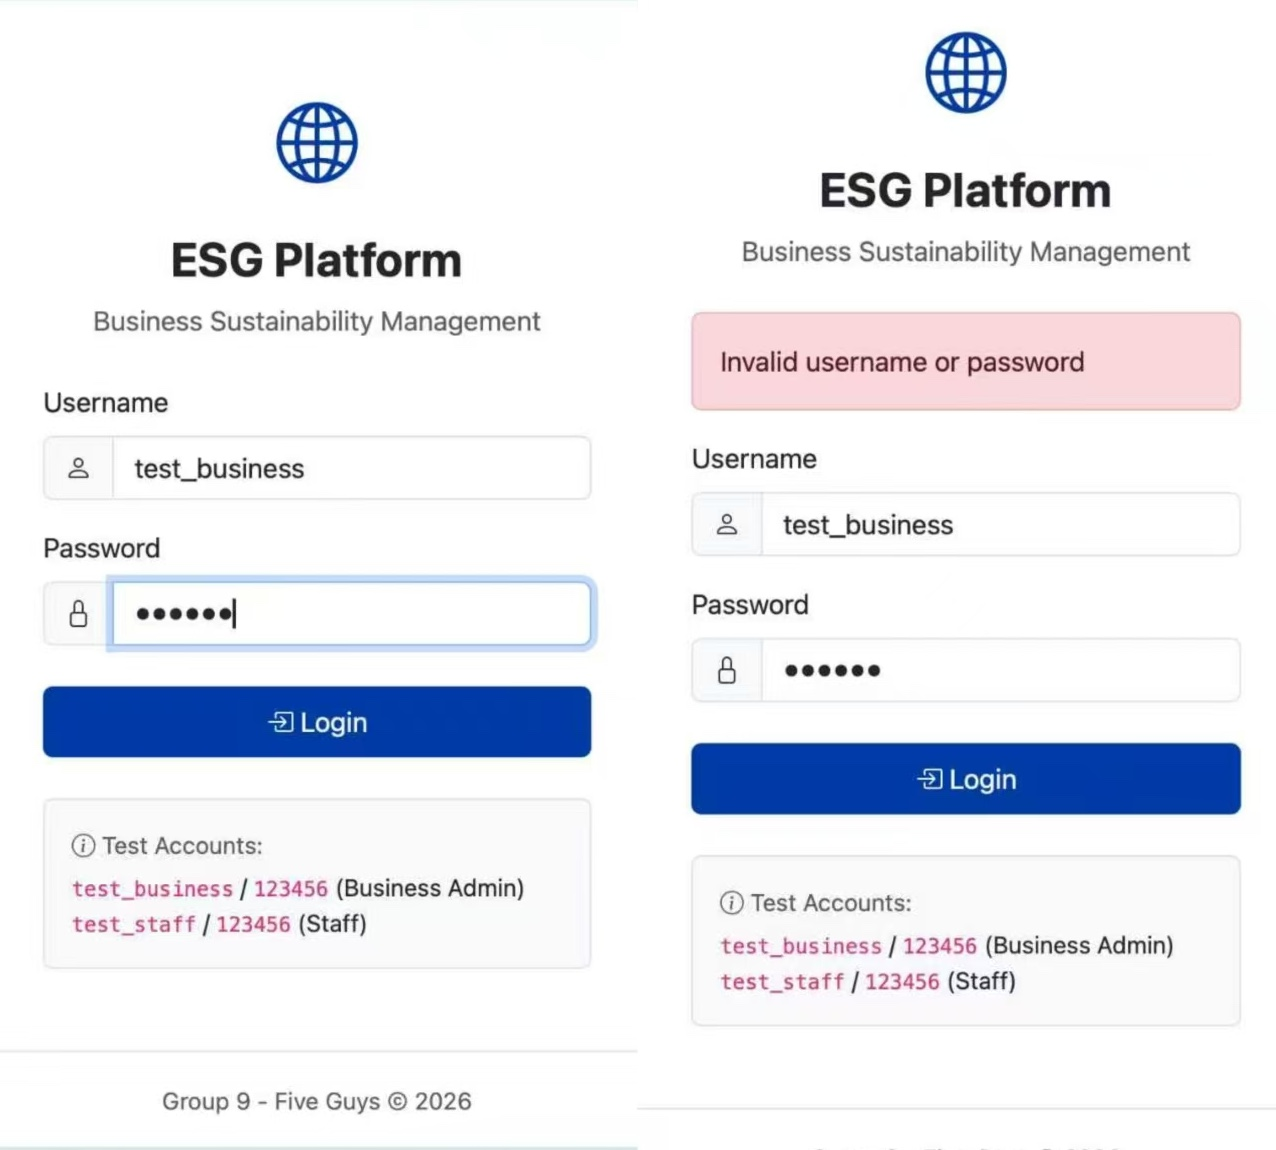
\includegraphics[width=0.50\textwidth]{login_page.jpg}
  \caption{Login page}
  \label{fig:login_page}
\end{figure}

\subsection{Test Accounts}
The following pre-configured accounts are available for testing. All accounts use the same URL and login page.

\begin{table}[H]
\centering\small
\begin{tabularx}{0.82\linewidth}{@{}lllX@{}}
\toprule
\textbf{Username} & \textbf{Password} & \textbf{Role} & \textbf{Access Scope} \\
\midrule
testbusiness & 123456 & HQ Manager & Full company-wide management \\
testregion & 123456 & Region Manager & Assigned region monitoring \\
teststaff & 123456 & Store Staff & Own store data entry \\
\bottomrule
\end{tabularx}
\caption{Pre-configured test accounts}
\end{table}

\subsection{Navigation and Layout}
Once logged in, users access all platform functions through the left sidebar. The sidebar lists the following modules in order: Dashboard, Carbon Tracking, Waste Management, Reports, Alerts, Training, ESG Management, Compliance Score, Anomaly Detection, User Management, and Audit Log. Not all entries are visible to every role -- lower-level users such as Store Staff only see the modules relevant to their responsibilities, while HQ Managers and Admins have access to the full list shown in Figure~\ref{fig:sidebar}. When there are unread alerts, a notification badge appears on the Alerts item. Across all pages, common interaction elements include data tables, filter controls, modal forms, summary cards, and charts.

\begin{figure}[H]
  \centering
  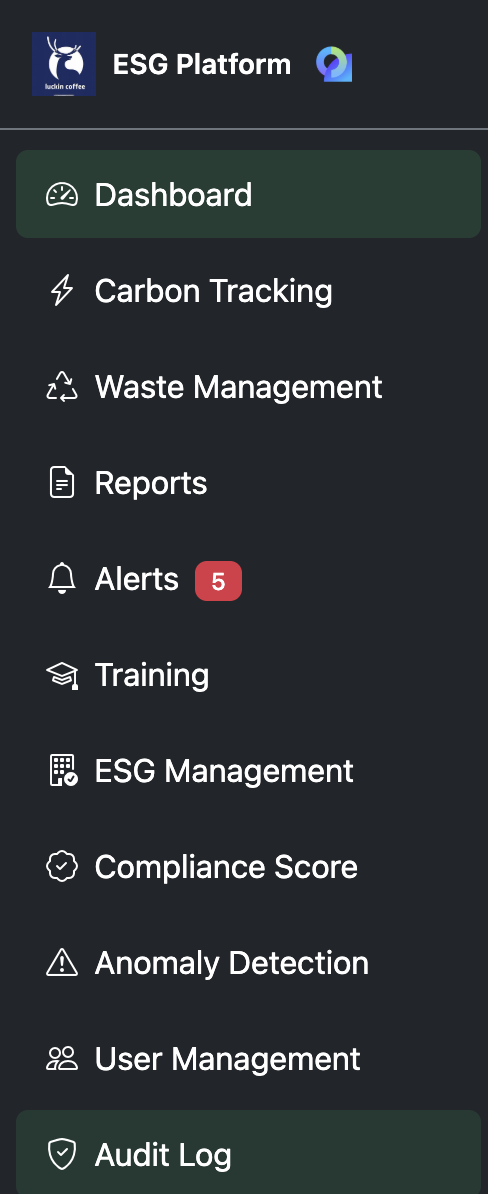
\includegraphics[width=0.22\textwidth]{sideBar.png}
  \caption{Navigation sidebar as seen by the Admin role (all menu items visible)}
  \label{fig:sidebar}
\end{figure}


\section{Role and Feature Overview}

\begin{table}[h]
\centering
\scriptsize
\begin{tabularx}{\linewidth}{@{}p{0.14\linewidth}p{0.22\linewidth}p{0.18\linewidth}p{0.14\linewidth}X@{}}
\toprule
\textbf{Role} & \textbf{Main Operational Pages} & \textbf{Management Pages} & \textbf{Typical Scope} & \textbf{Important Restriction} \\
\midrule
Store Staff & Dashboard, Carbon, Waste, Reports, Training & Minimal & Own store & No high-level management pages; stricter edit/delete limits \\
Region Manager & Dashboard, Carbon, Waste, Reports, Training, Alerts, Compliance, Anomaly Detection & Monitoring and review & Assigned region & Cannot manage users or create company policies \\
HQ Manager & Core pages plus Alerts, Compliance, ESG Management, User Management, Audit Log & Company-wide management & Company-wide & Handles governance content and threshold configuration \\
Admin & Similar to HQ Manager with broader authority & Full administration & Platform-wide & Can manage users more broadly and inspect audit activities \\
\bottomrule
\end{tabularx}
\caption{Role and access scope overview}
\end{table}


\section{Shared Core Workflows}

\subsection{Dashboard Review}
The dashboard acts as the main overview page after login. It shows summary cards for annual carbon emissions, total waste, recycling rate, and report count. It also includes charts for monthly carbon trend, carbon by category, and waste composition, plus an SDG 12 panel that connects system data with broader sustainability indicators \cite{un_sdg12}. The charts support drilldown and deeper inspection and the visible data scope depends on the user's role.

\begin{figure}[H]
  \centering
  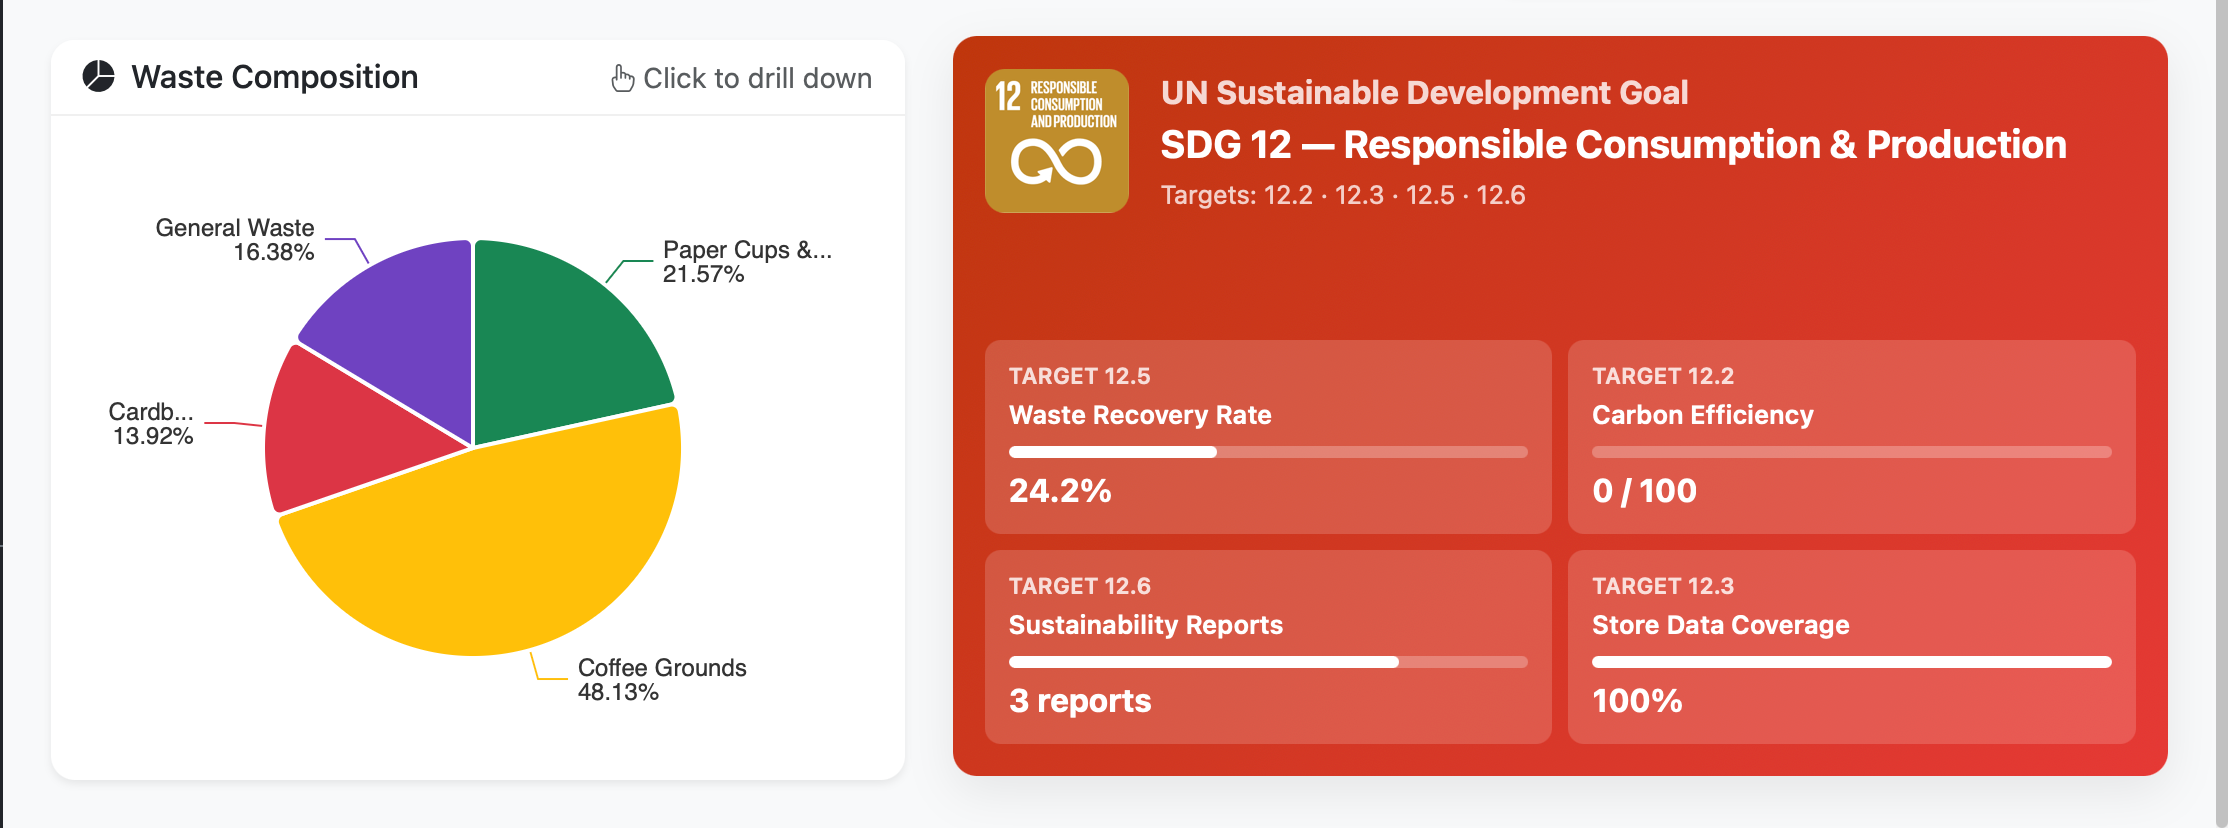
\includegraphics[width=0.78\textwidth]{SDG_panel.png}
  \caption{SDG 12 alignment panel on the dashboard}
  \label{fig:SDG_panel}
\end{figure}


\subsection{Carbon Tracking}
The carbon tracking page is used to record carbon-related operational activity. Users can create records, review existing entries, and in some cases edit or delete recent entries.

\begin{figure}[H]
  \centering
  \begin{minipage}[b]{0.60\textwidth}\centering
    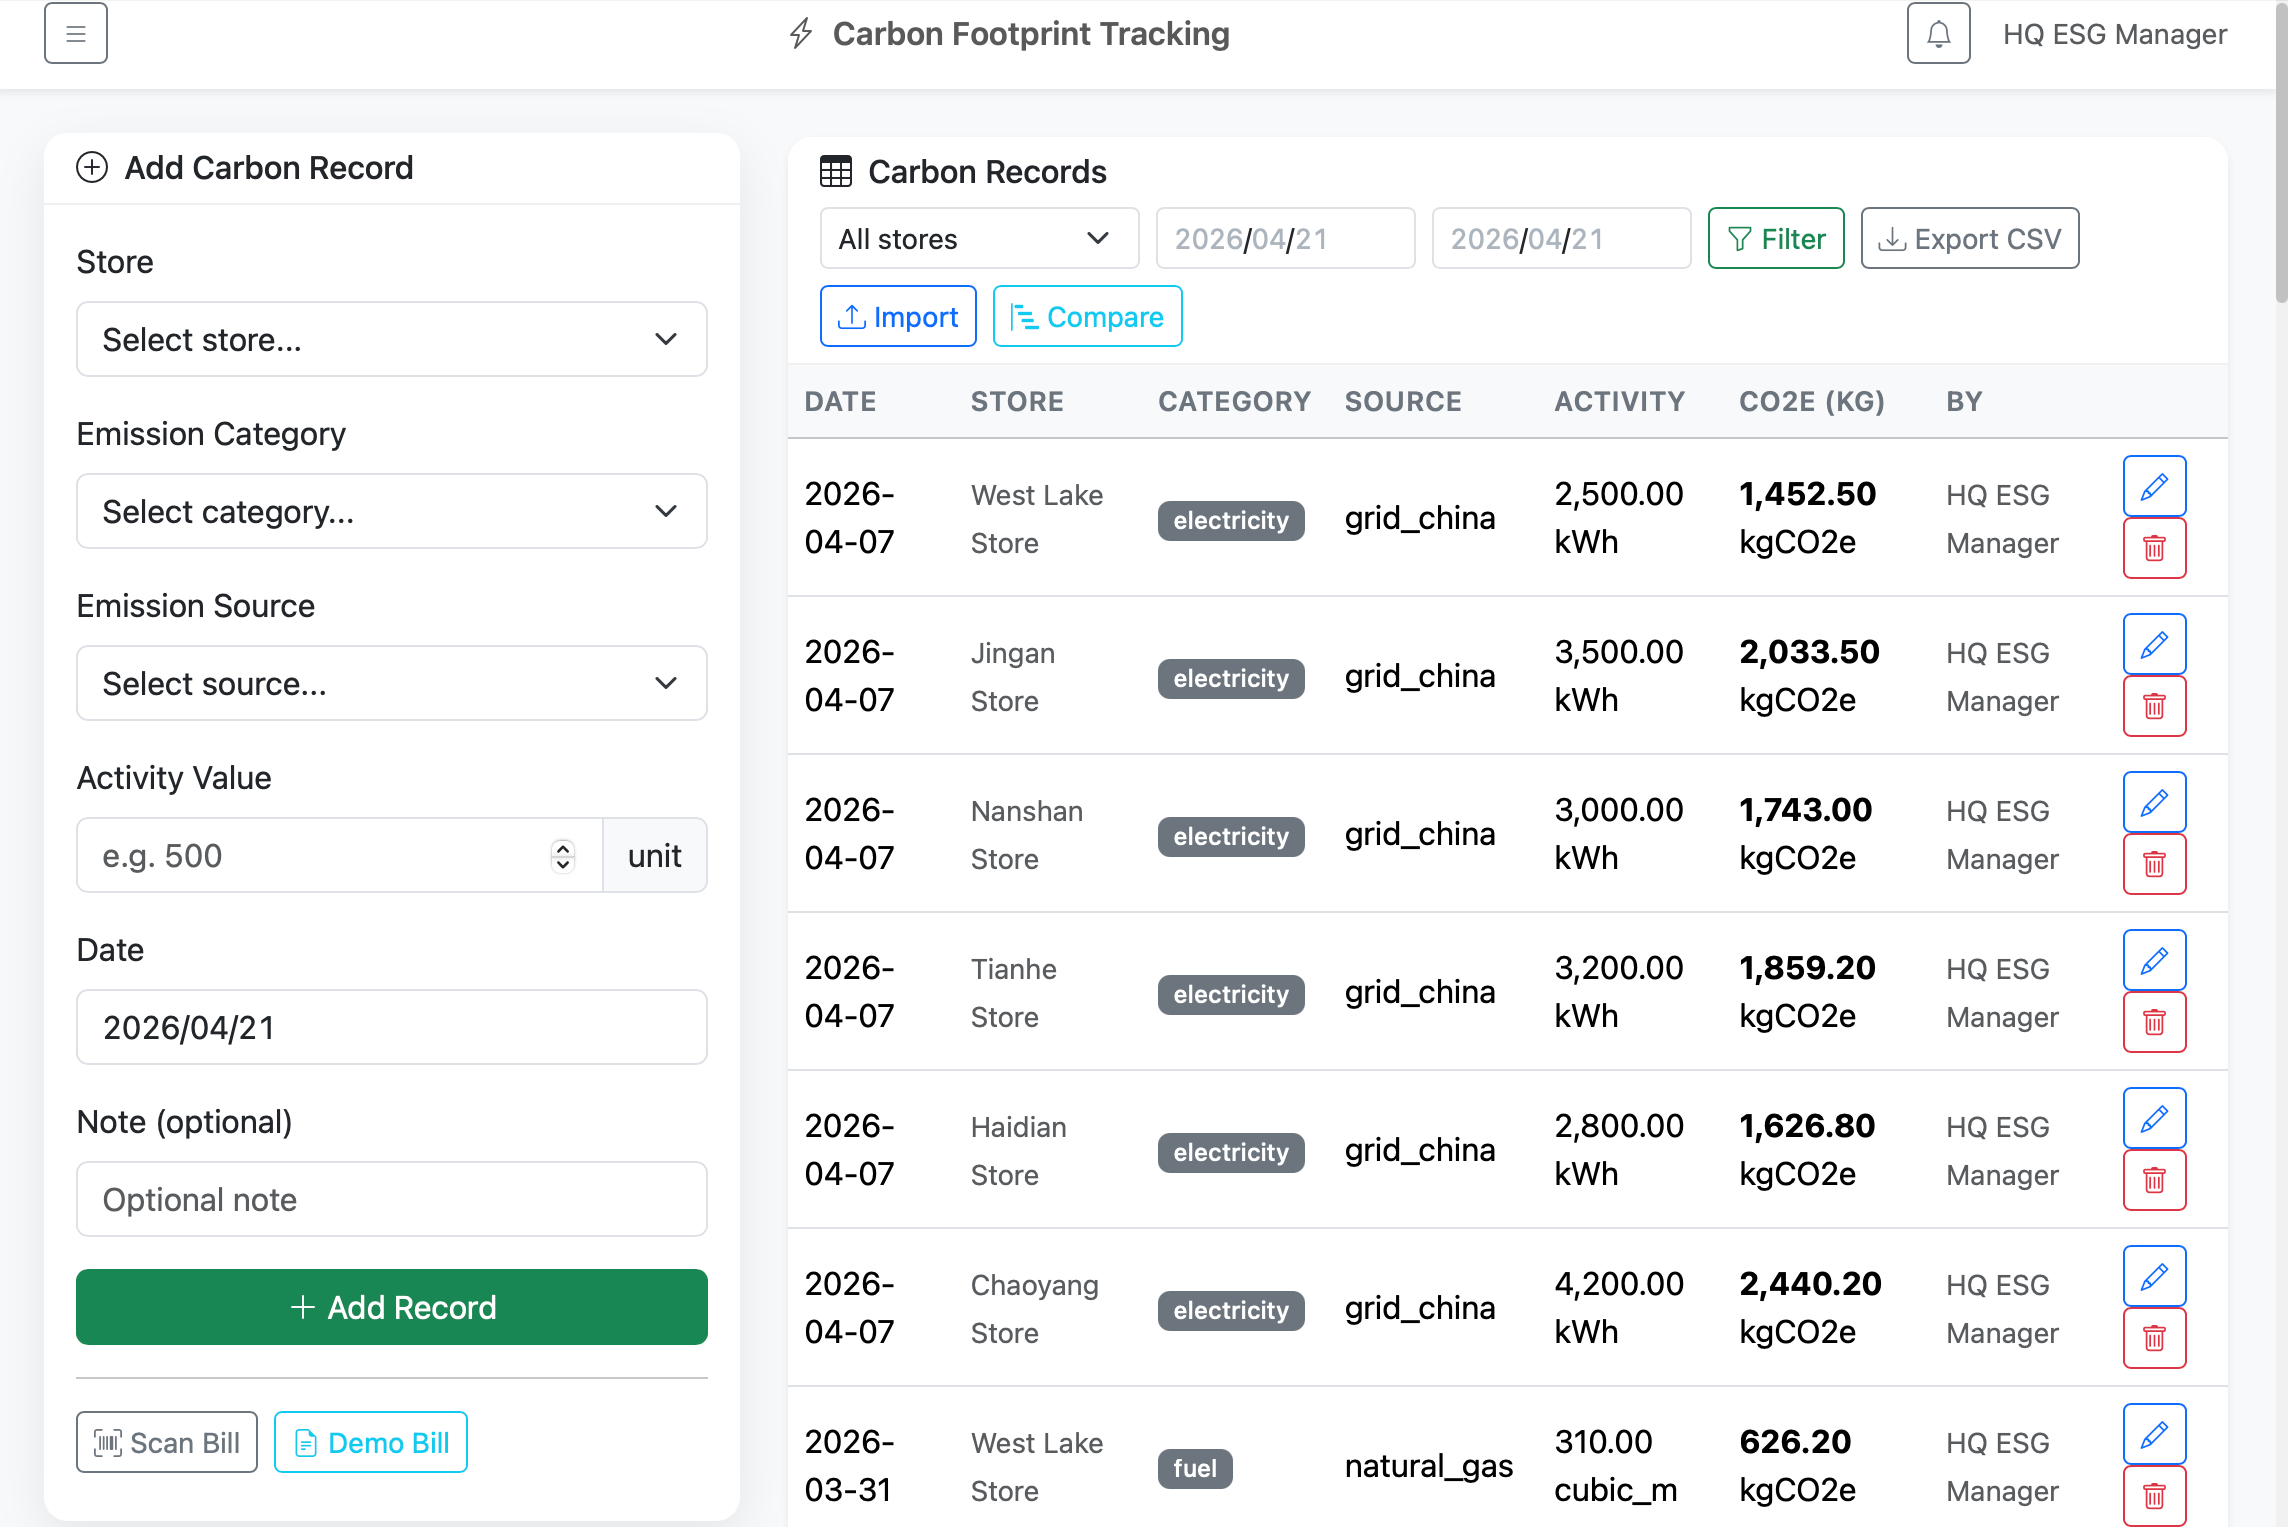
\includegraphics[width=\linewidth]{carbon_tracking.png}
  \end{minipage}\hfill
  \begin{minipage}[b]{0.36\textwidth}\centering
    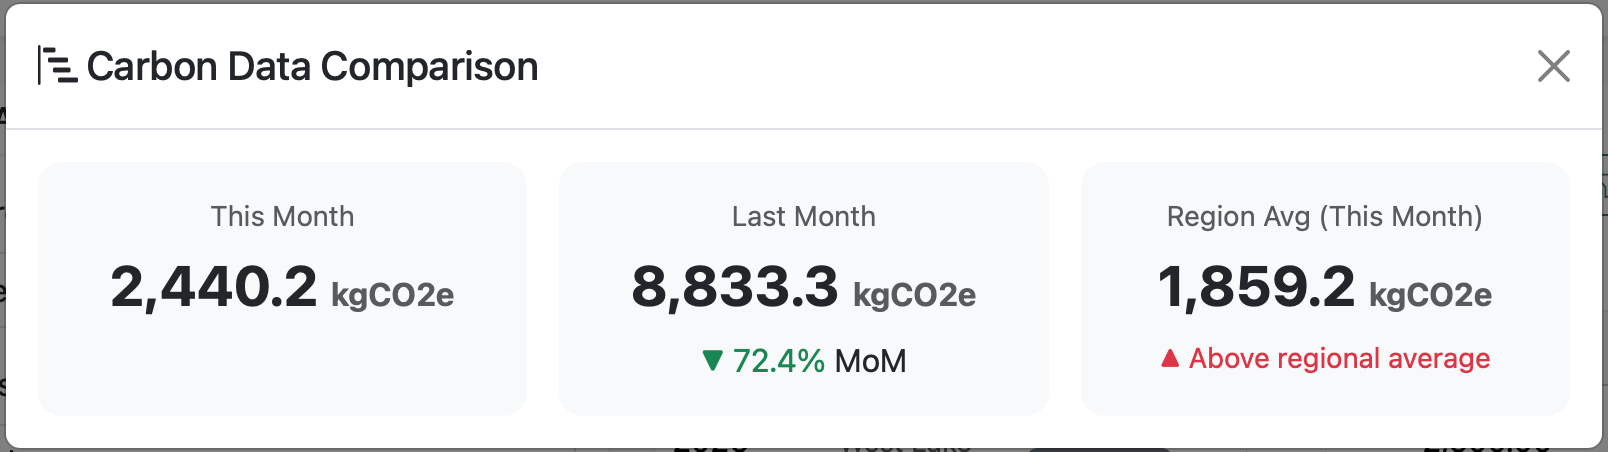
\includegraphics[width=\linewidth]{carbon_comparison.png}
  \end{minipage}
  \caption{Carbon tracking page (left) and monthly comparison view (right)}
  \label{fig:carbon}
\end{figure}

To add a new record, open the Carbon Tracking page from the sidebar, click the add button, fill in the required fields, and submit. The submitted record appears in the table immediately. Users with lower-level roles are limited to their own store's data scope, and store staff may face tighter time windows for editing or deleting records. All carbon data submitted through this page later contributes to dashboard charts, sustainability reports, and compliance-related scoring.

\subsection{Waste Management}
The waste management page is used to record waste generation, recycled quantity, category, source, and disposal information. Like carbon tracking, it is both an operational input page and an analytical data source for later reporting and monitoring.

\begin{figure}[H]
  \centering
  \begin{minipage}[b]{0.60\textwidth}\centering
    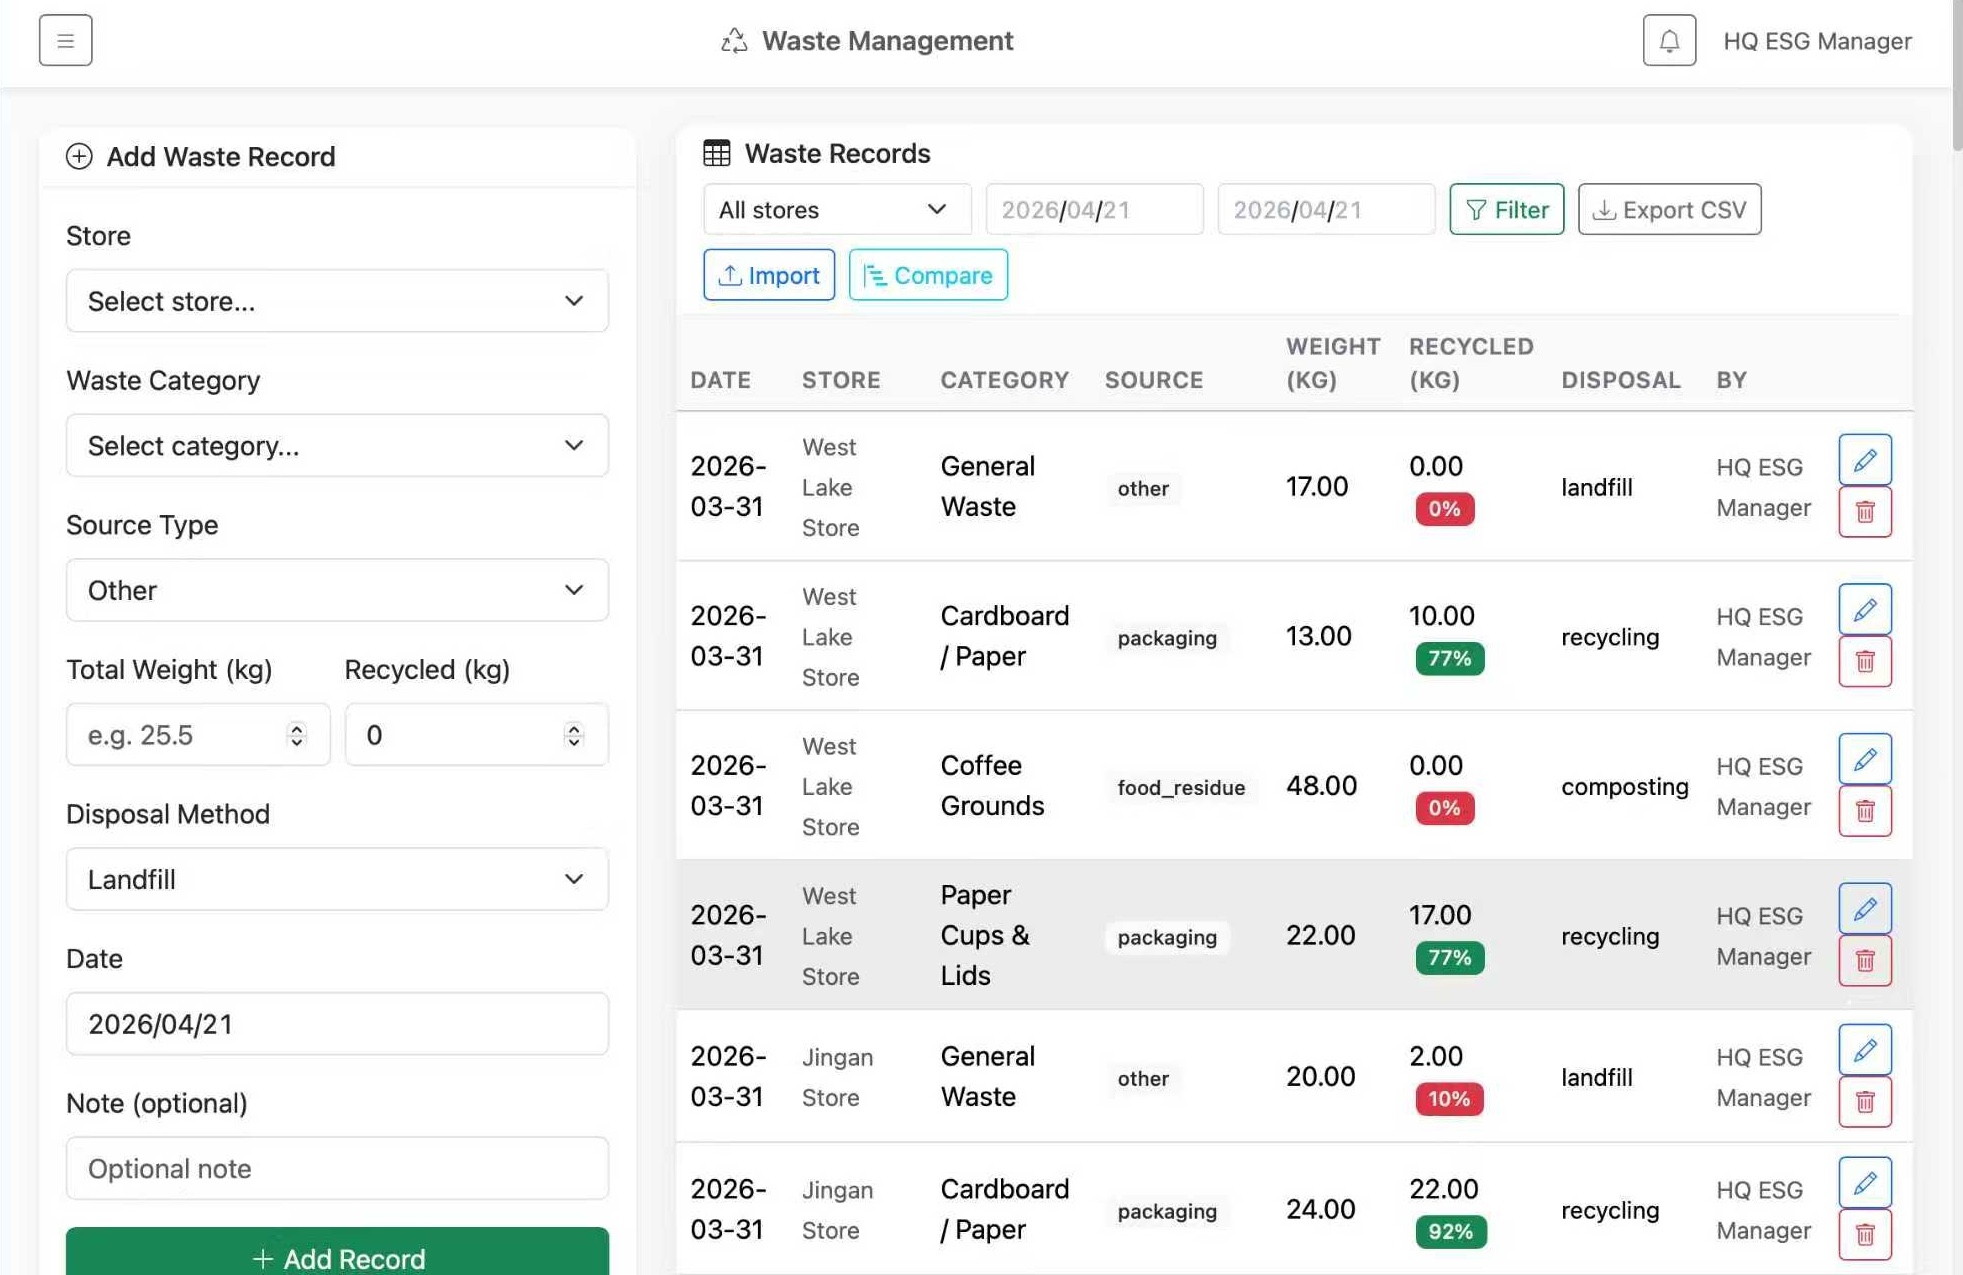
\includegraphics[width=\linewidth]{waste_management.jpg}
  \end{minipage}\hfill
  \begin{minipage}[b]{0.36\textwidth}\centering
    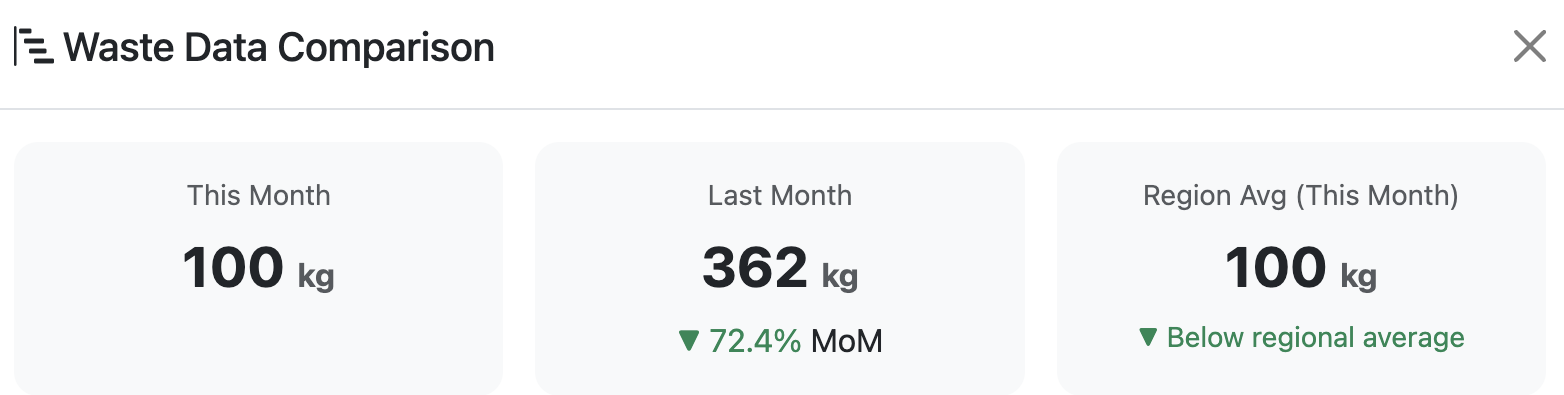
\includegraphics[width=\linewidth]{waste_comparison.png}
  \end{minipage}
  \caption{Waste management page with inline entry form and records table (left) and month-on-month comparison modal (right)}
  \label{fig:waste}
\end{figure}

Users can add, review, and manage waste records from this page. To log a new entry, click the add button to open the data entry form, fill in fields such as waste category, total weight, recycled quantity, source, disposal method, and date, then submit. The recycled quantity must remain logically consistent with the total waste volume -- the system will reject entries where recycled weight exceeds total waste. Like carbon tracking, the data scope follows the user's organisational role, and the records feed into dashboards, reports, and later monitoring analysis. The page also provides a month-on-month comparison view accessible via the Compare button, showing this month's total waste, the previous month, and the regional average.

\subsection{Sustainability Reports}
The Reports page allows users to generate sustainability reports for a selected time range. The user provides a title, report type, and date range, then the system generates a structured report and stores it in the report list. Users can preview the report content, export it as PDF, and optionally request AI-generated ESG analysis in line with standard sustainability reporting practices \cite{gri_standards}.

\begin{figure}[H]
  \centering
  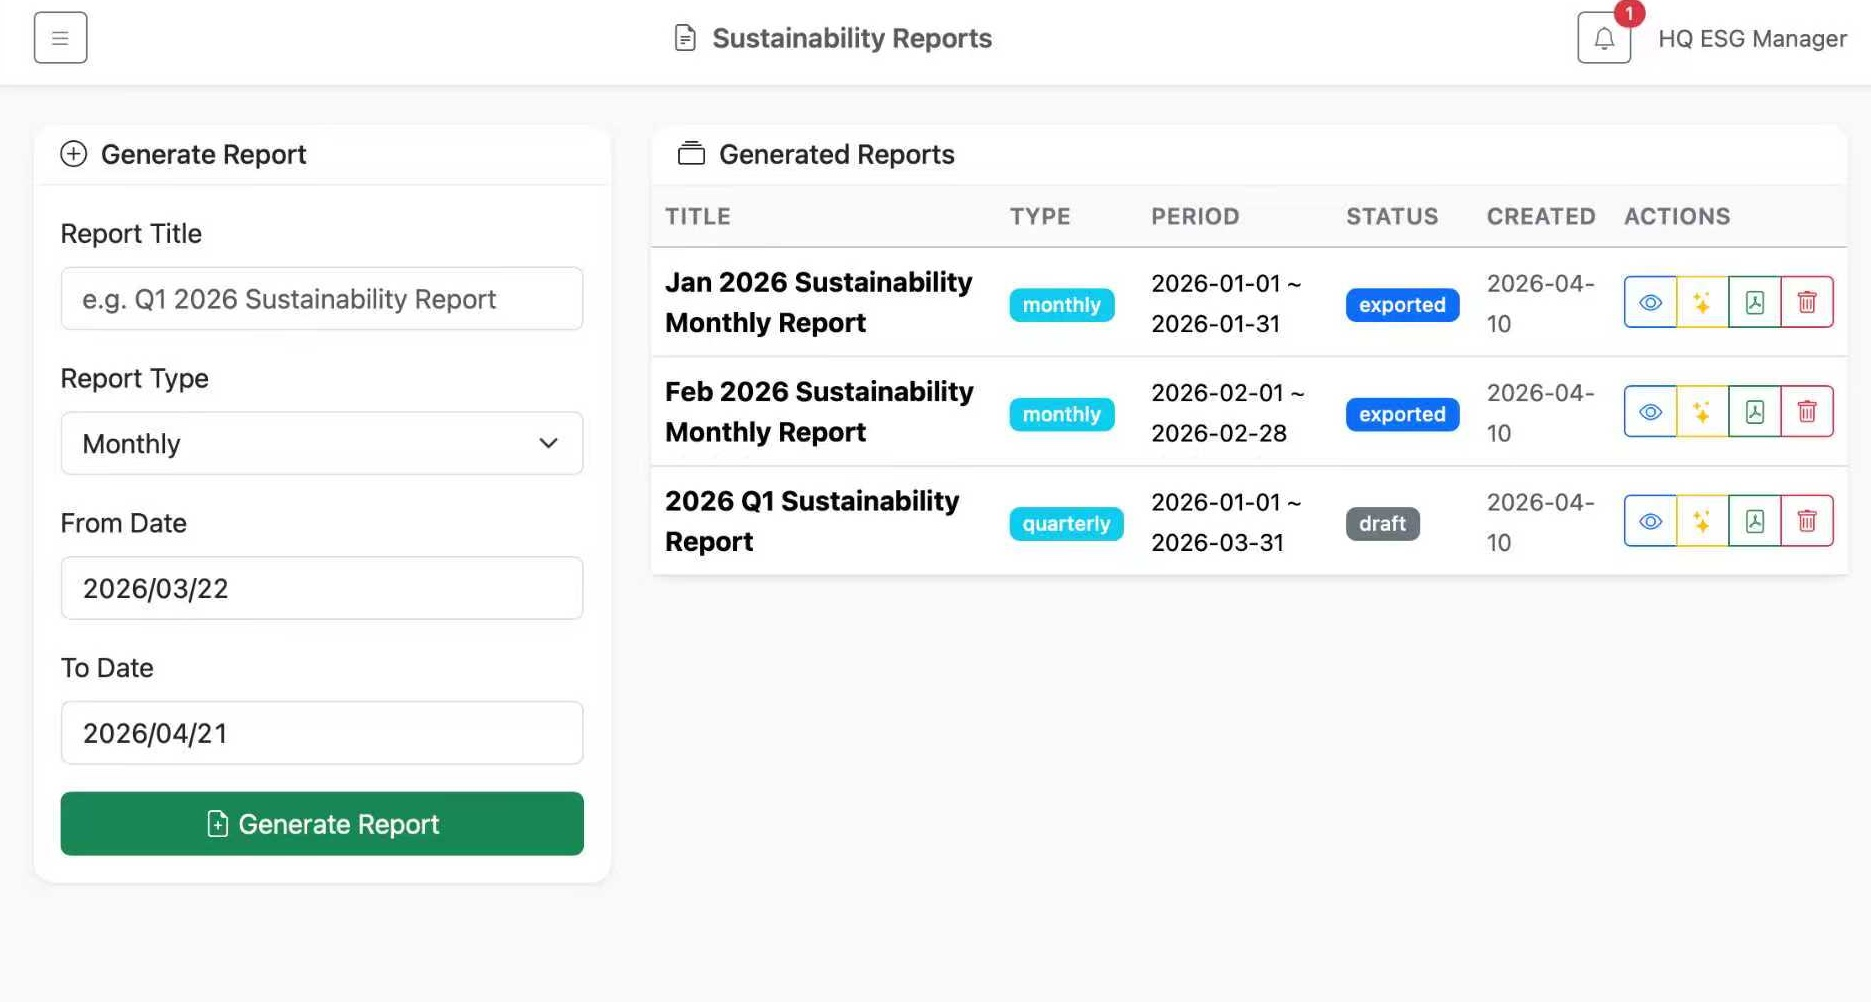
\includegraphics[width=0.65\textwidth]{reports_page.jpg}
  \caption{Sustainability reports page}
  \label{fig:reports_page}
\end{figure}

To generate a report, open the Reports page, enter a title, choose the report type and period, and click \texttt{Generate Report}. The system creates and stores the report, which then appears in the report list. From there, users can open the item to preview its content, export it as a PDF, or request AI-generated ESG analysis. AI-generated analysis is subject to service availability in the deployment environment.

\subsection{Training Records}
The Training page records staff sustainability training sessions. To log a new session, fill in the course name, type, store, trainee, duration, completion date, score, and status, then submit. Course type and status fields help classify and filter records later. The right panel displays annual summary statistics -- session count, total hours, unique trainees, and average score -- alongside a filterable training-record table.

\begin{figure}[H]
  \centering
  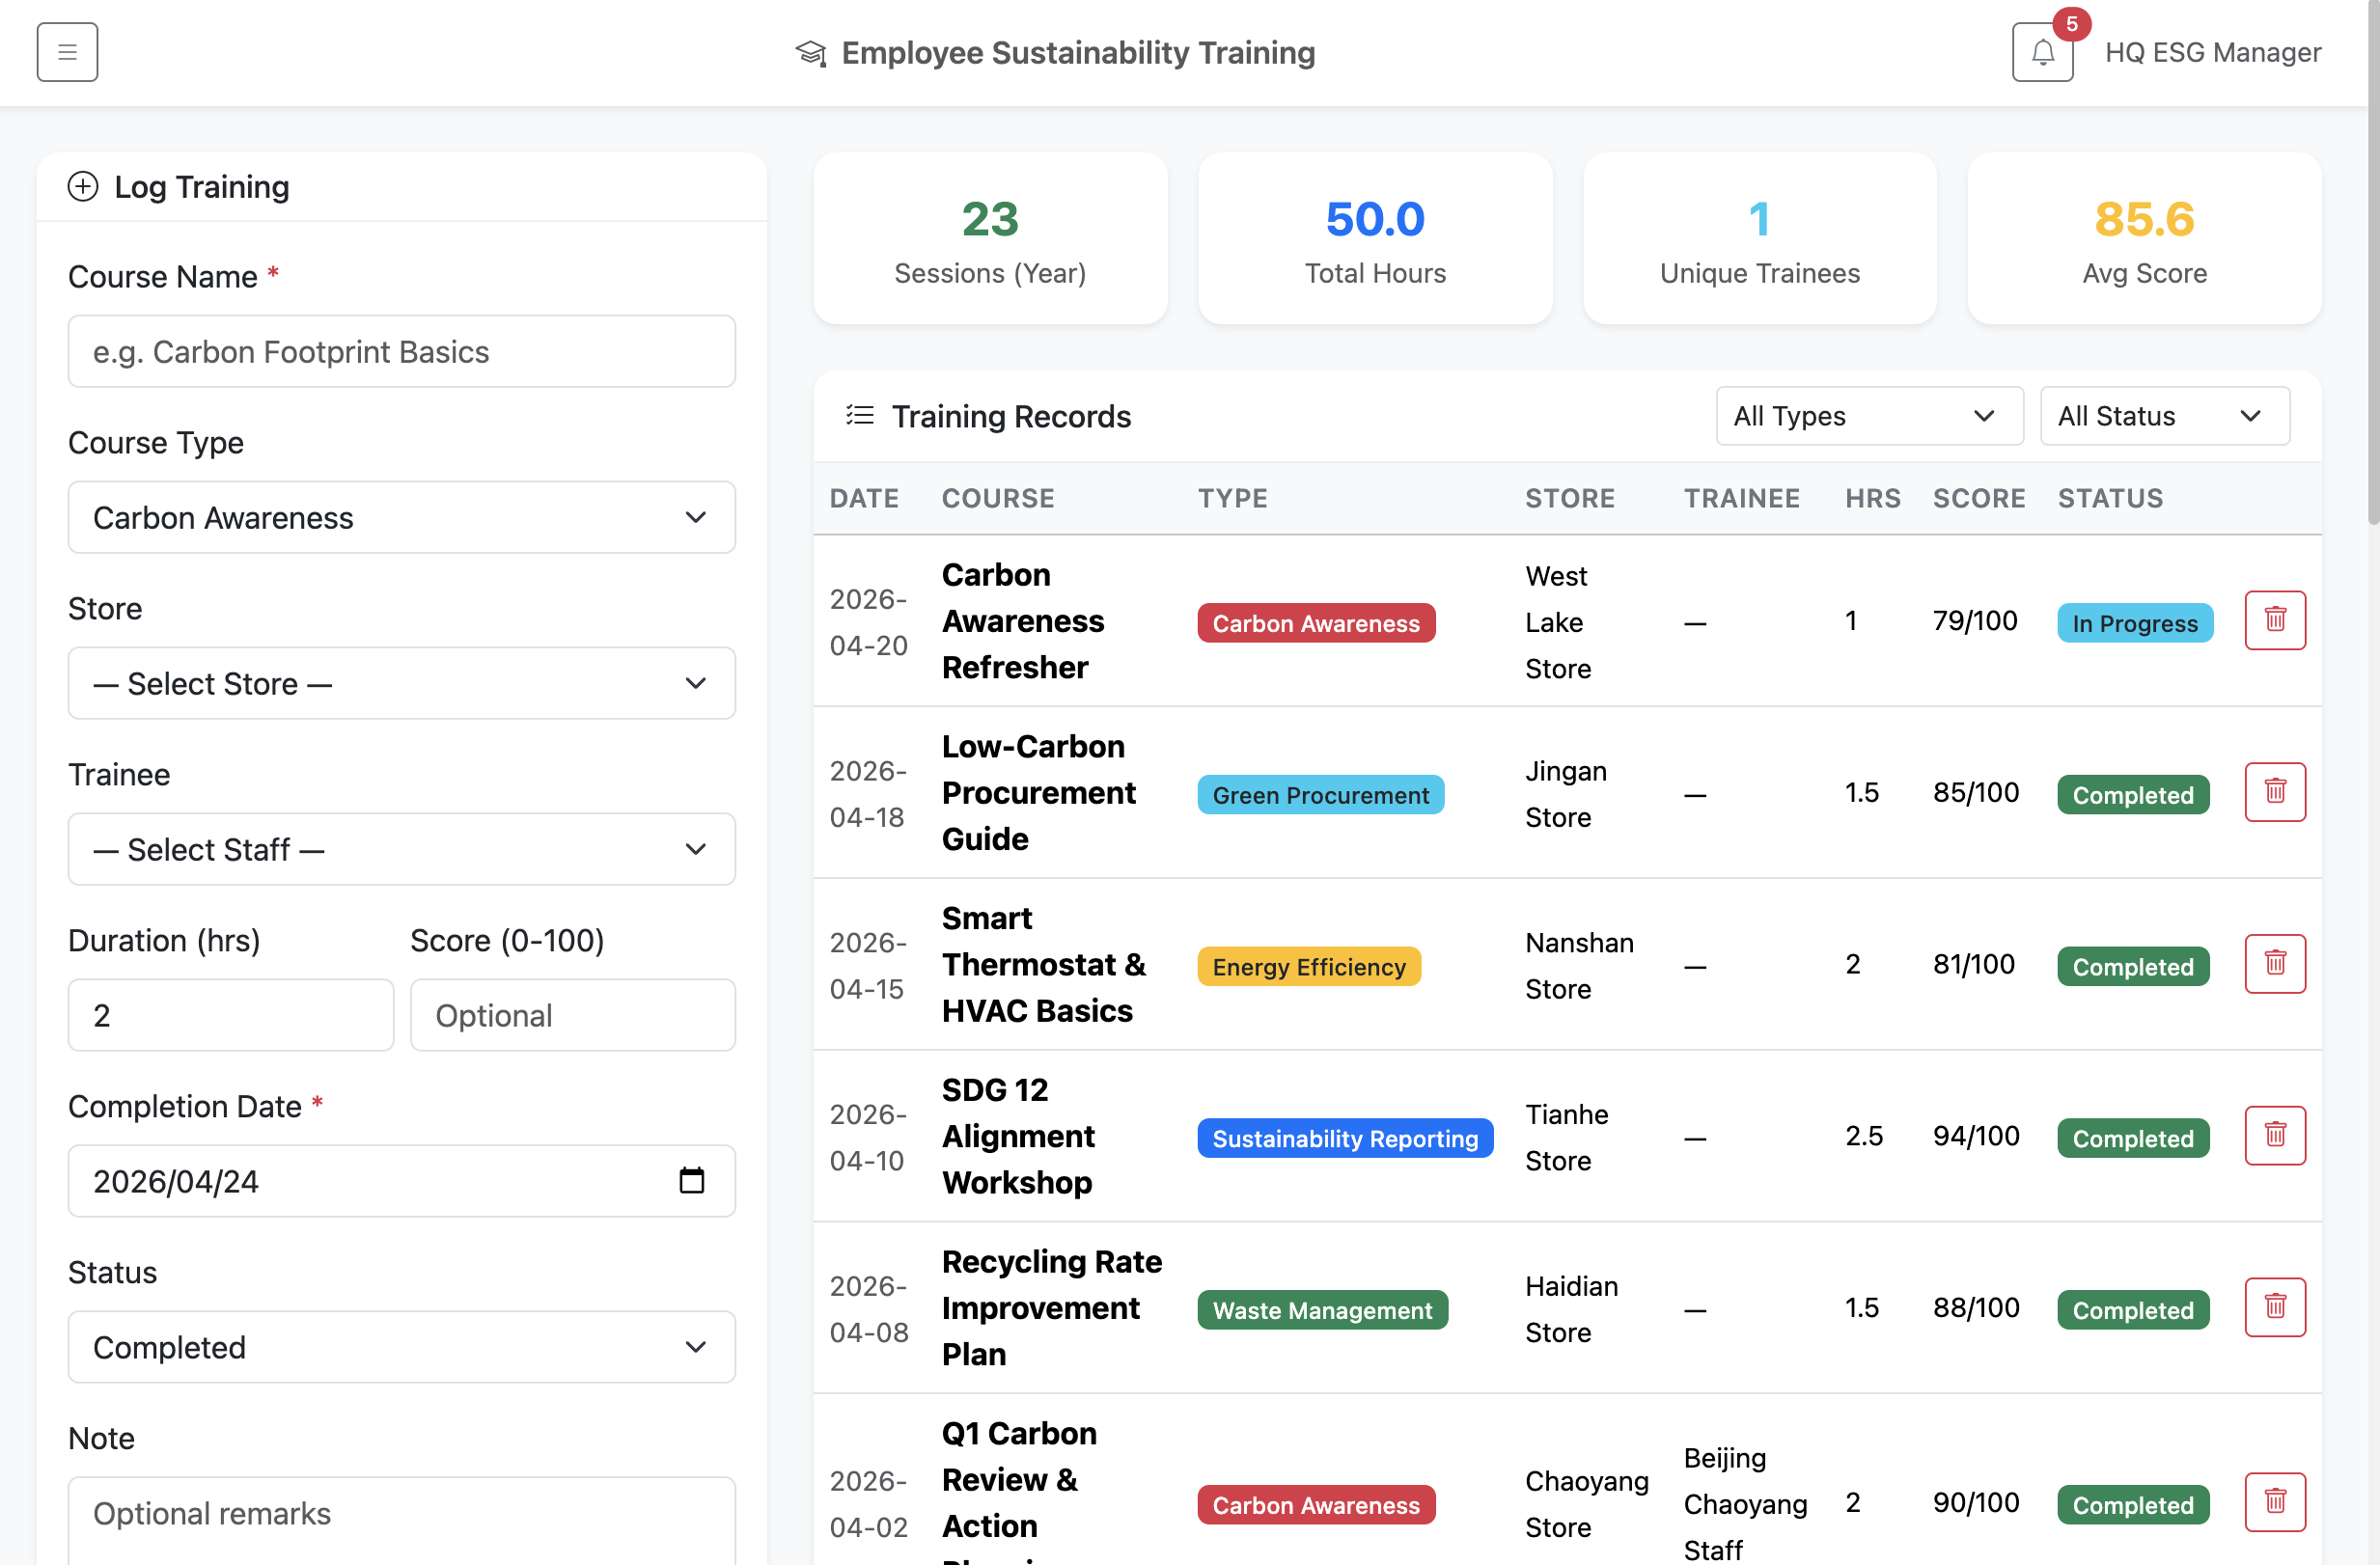
\includegraphics[width=0.85\textwidth]{training_page.png}
  \caption{Training page showing the log form (left), summary statistics, and training records table}
  \label{fig:Training_page}
\end{figure}


\section{Store Staff Guide}

Store staff are the most operationally focused users on the platform. Their primary responsibility is to record day-to-day sustainability data for their own store, contributing to consistent data collection across the organisation. The main pages used by store staff are Dashboard, Carbon Tracking, Waste Management, Reports, and Training.

A typical store staff workflow begins by reviewing the dashboard after login, then entering new carbon records for ongoing store operations, followed by waste records with accurate recycling values. Reports can be generated or reviewed as needed for the current period, and training activities can be logged or checked at any time.

Store staff do not have access to threshold configuration, compliance scoring, anomaly detection, user management, or audit logs. Their visible data is restricted to their own store, and edit or delete operations on submitted records may be subject to stricter time limits than higher-level roles.

\begin{figure}[H]
  \centering
  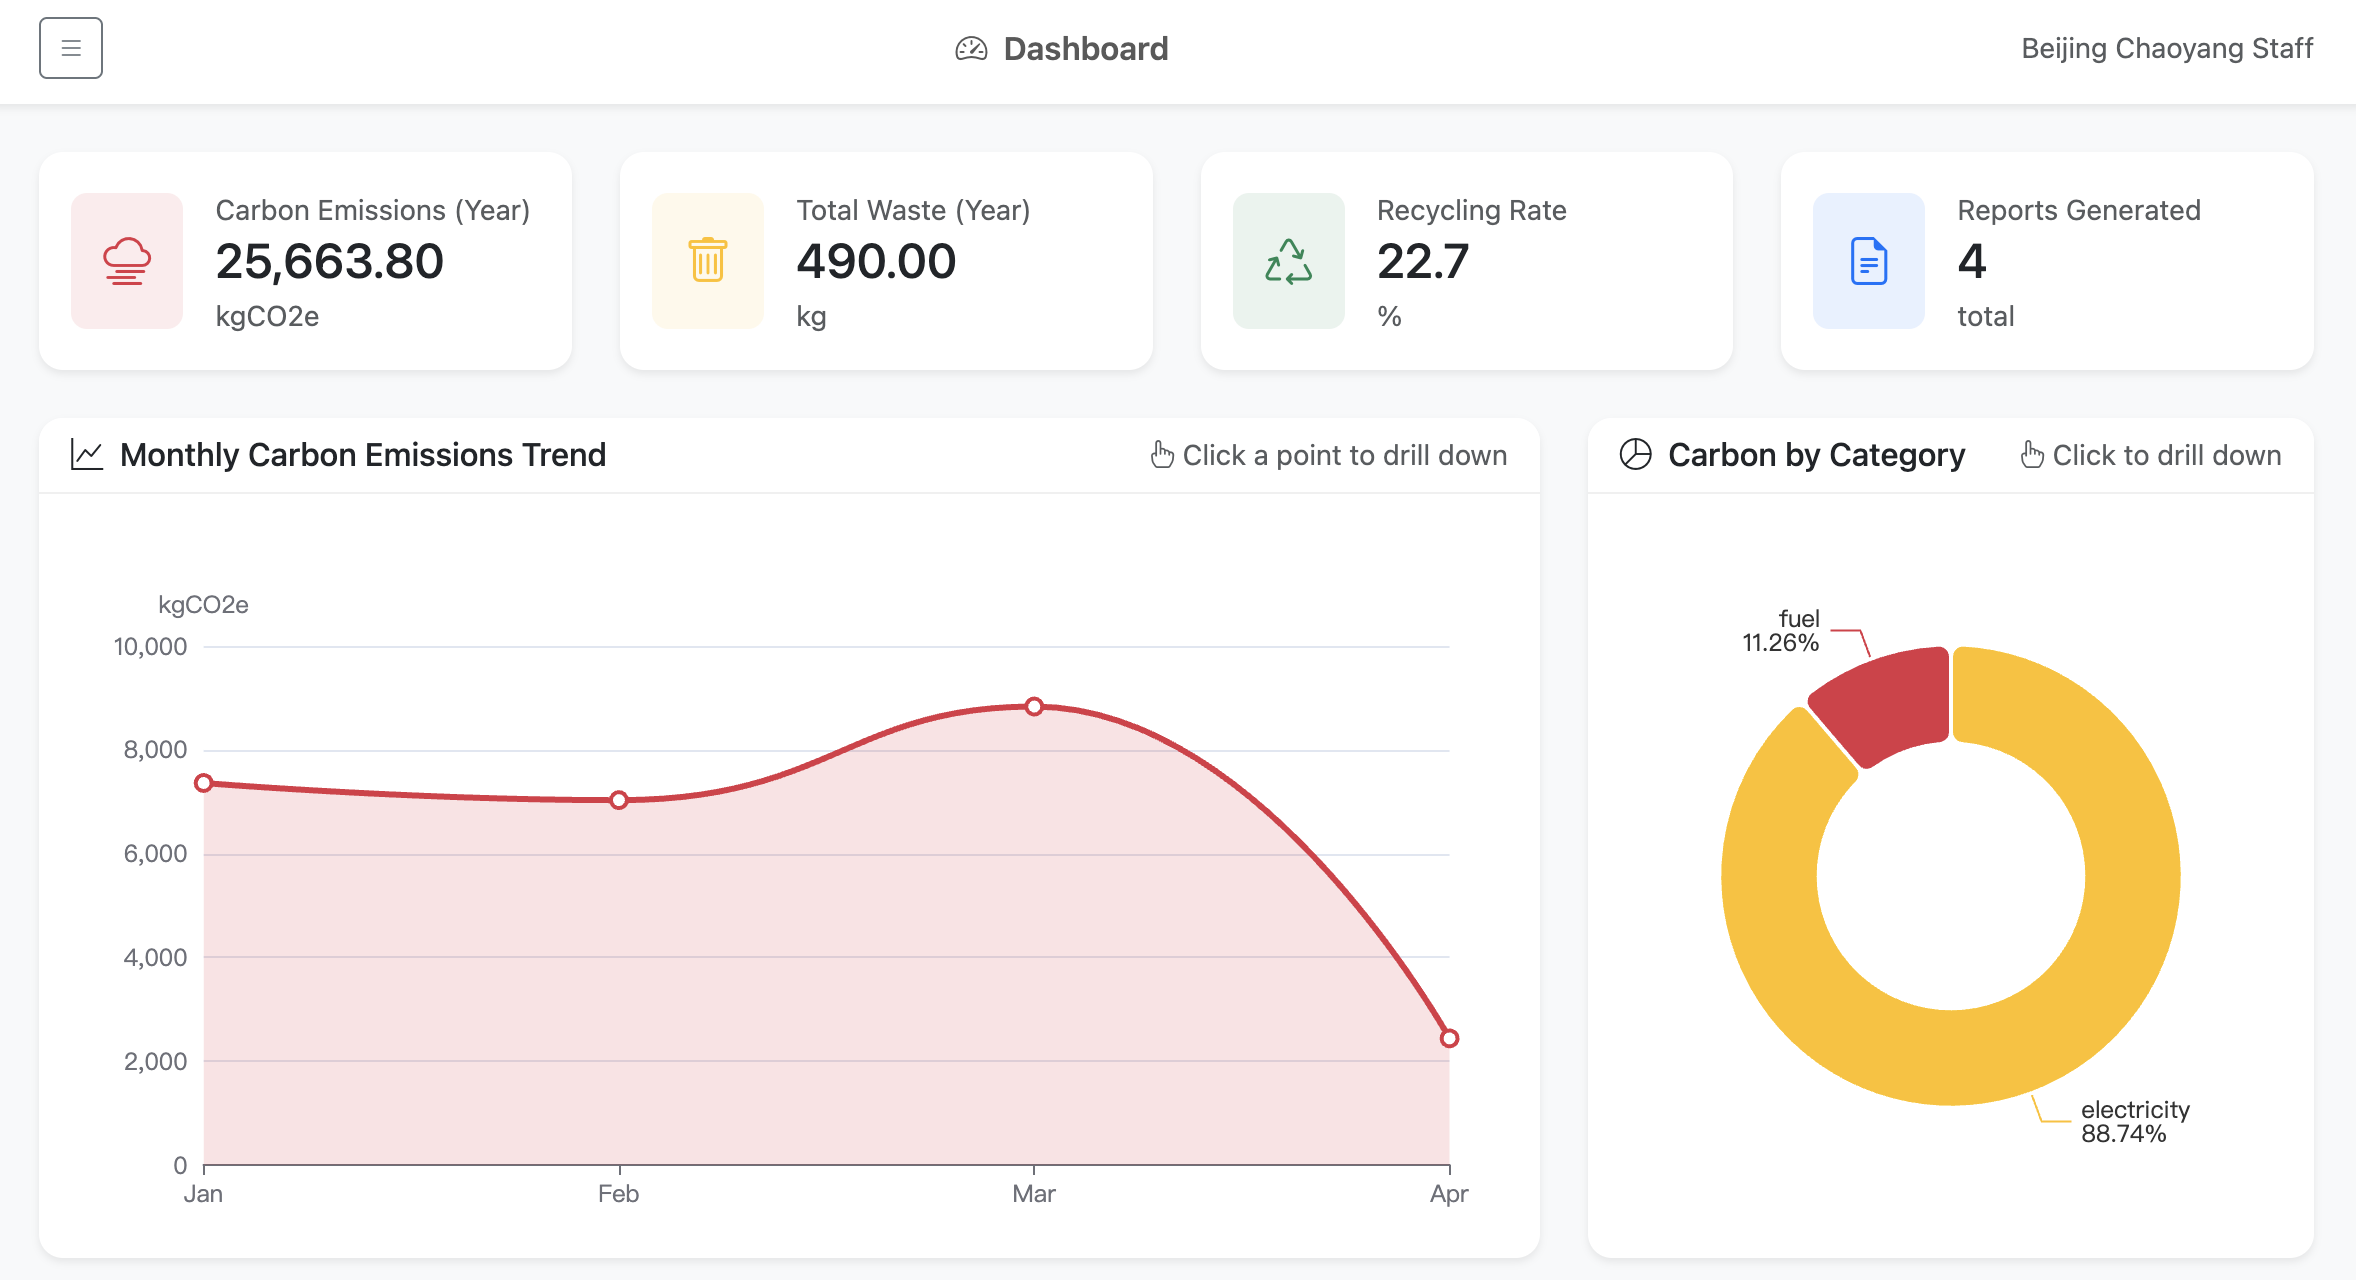
\includegraphics[height=4.5cm]{dashboard_staff.png}
  \hfill
  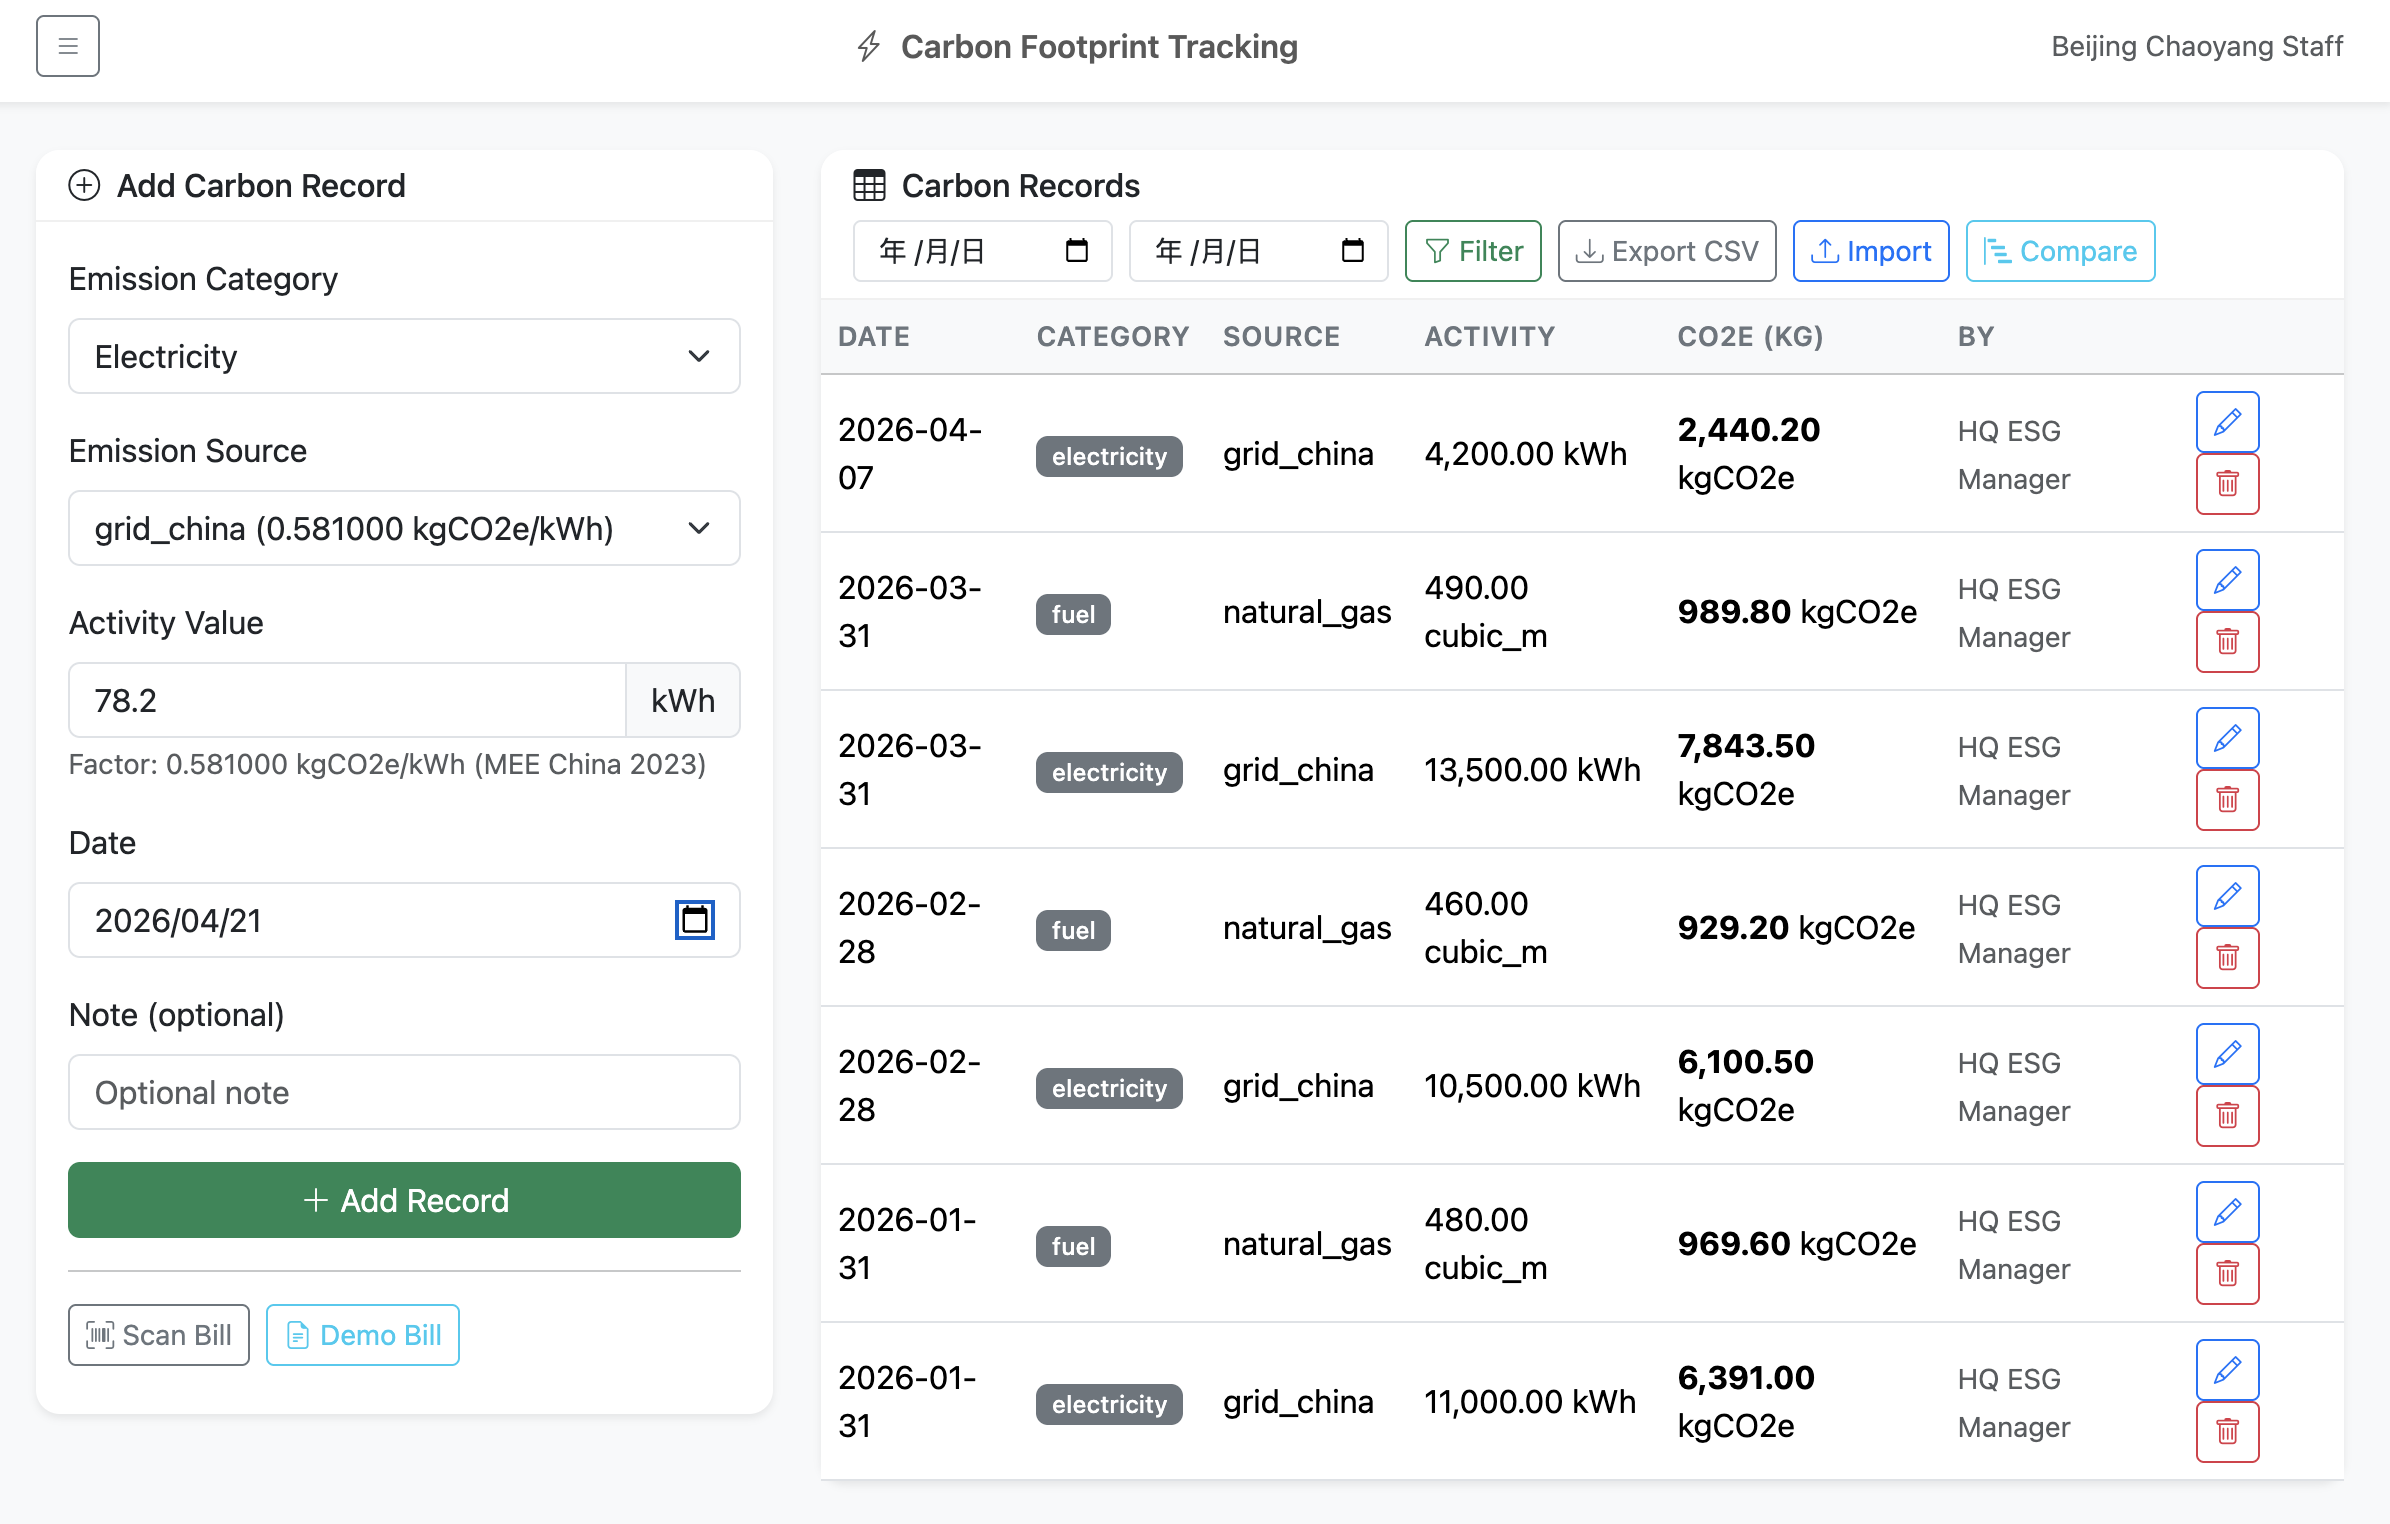
\includegraphics[height=4.5cm]{carbon_add_form.png}
  \caption{Store staff dashboard showing store-scoped data (left) and carbon record entry form (right)}
  \label{fig:staff-view}
\end{figure}


\section{Region Manager Guide}
\label{sec:region}

Region managers supervise sustainability performance across multiple stores within their assigned region. Compared with store staff, they focus less on raw data entry and more on monitoring, comparison, and issue identification. In addition to the common pages available to all users, region managers can access Alerts, Compliance Score, and Anomaly Detection, which help them identify unusual values, assess ESG readiness, and monitor whether stores are meeting sustainability expectations.

\subsection{Alerts Page}
The Alerts page contains alert logs for monitoring threshold breaches. Depending on permissions, region managers can at least review logs, inspect metric values, and monitor whether issues have been noticed or marked as read.

\begin{figure}[H]
  \centering
  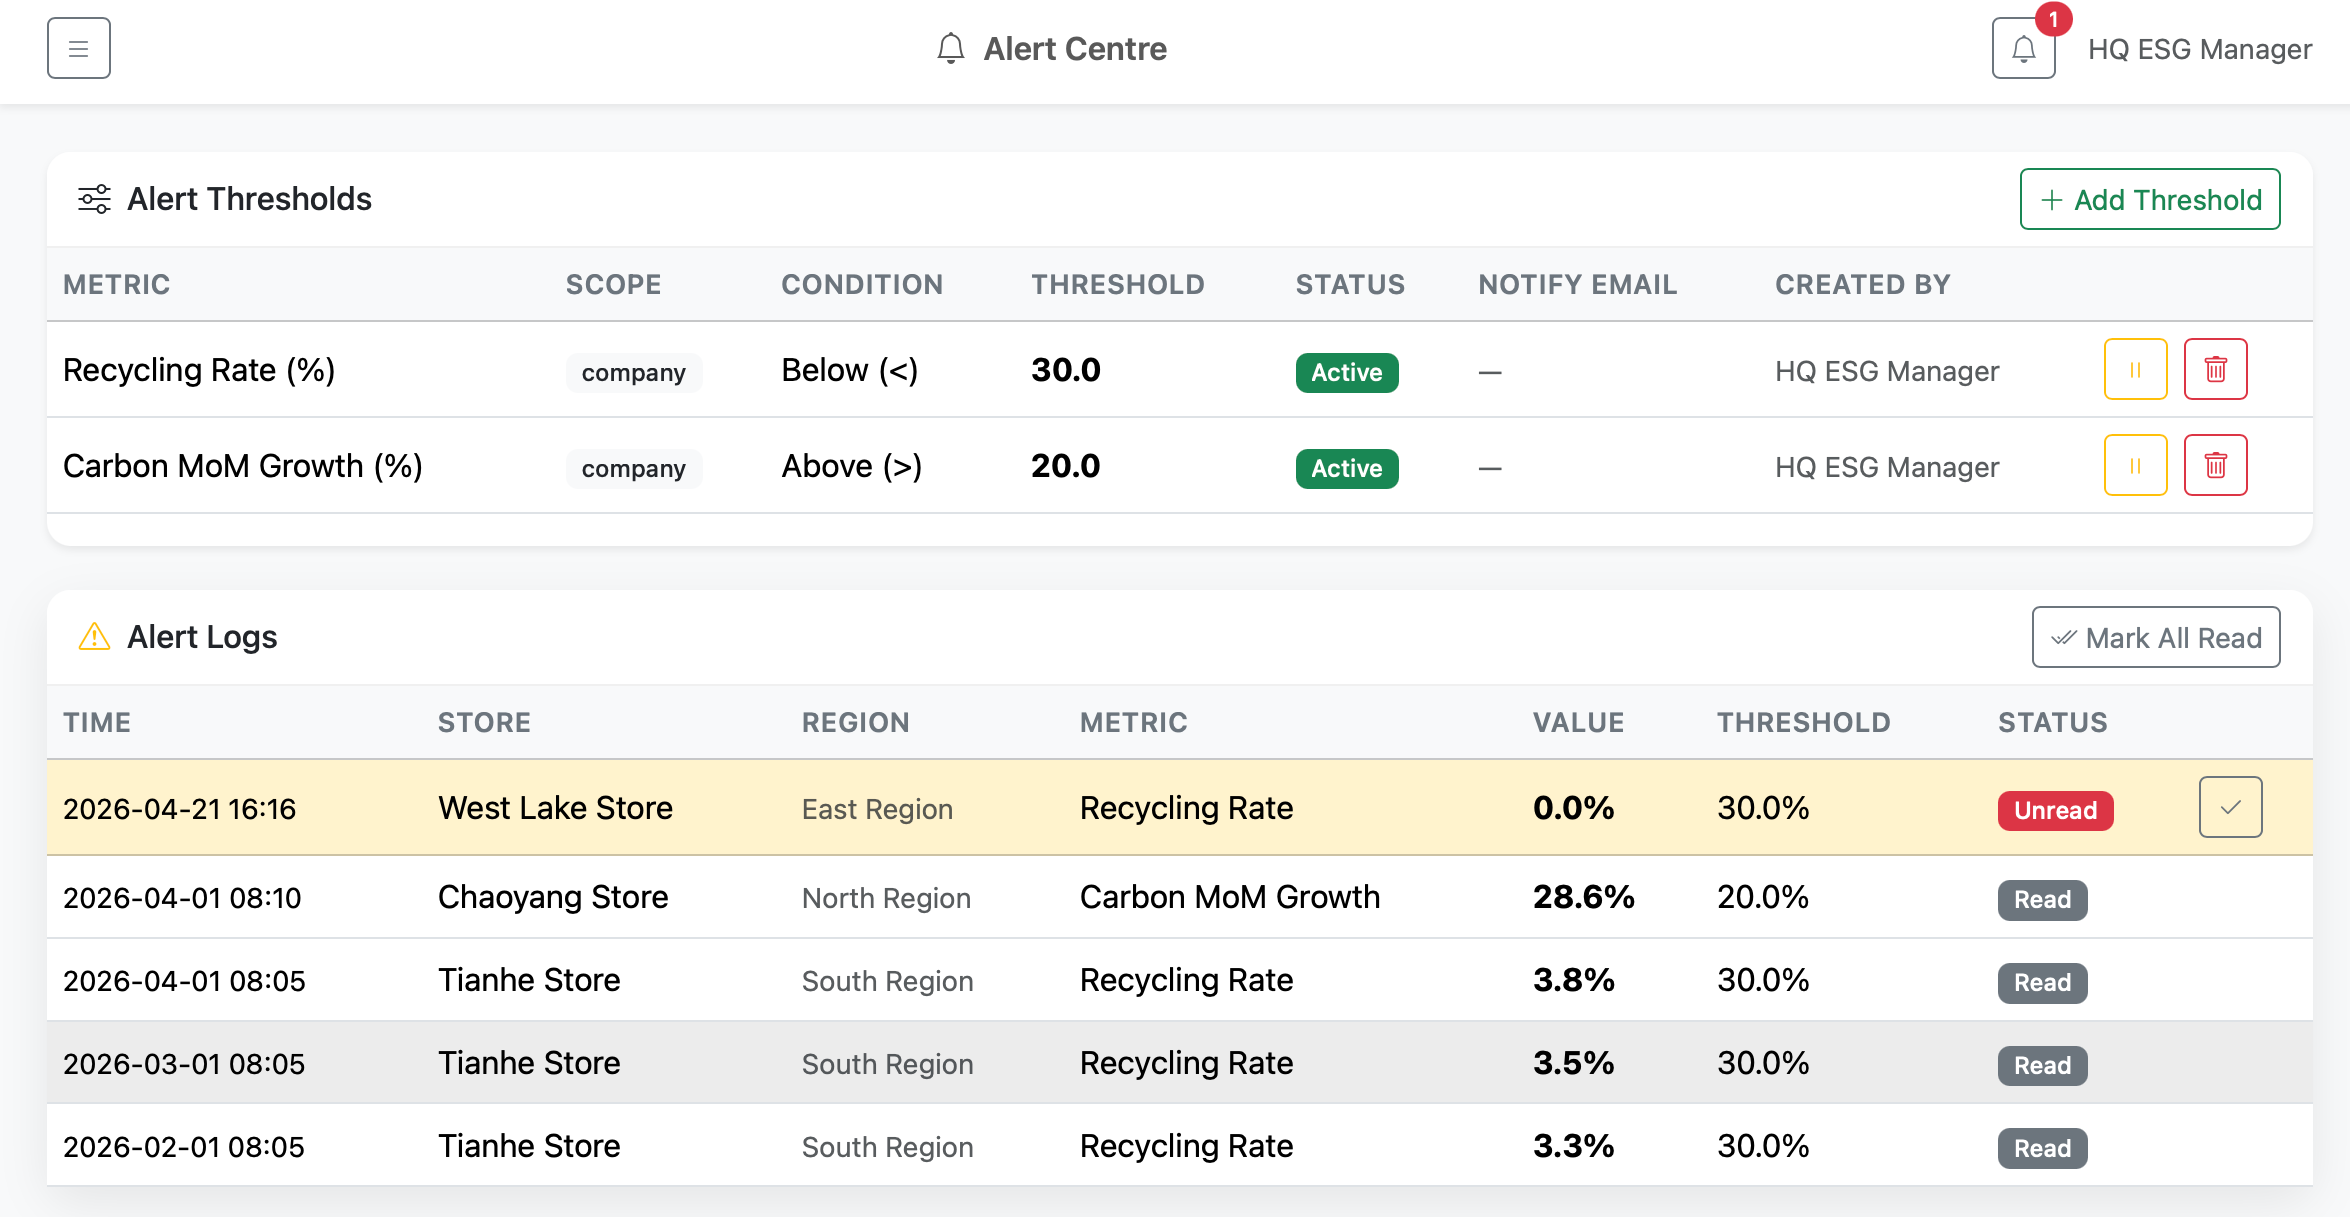
\includegraphics[width=0.65\textwidth]{alert_page.png}
  \caption{Alert Centre showing threshold rules and alert log entries}
  \label{fig:alert_page}
\end{figure}

\subsection{Compliance Score Page}
The Compliance Score page allows management users to calculate and review an ESG scorecard for a selected year. It includes an overall score gauge, a grade label, dimension breakdowns, and detailed metric rows. This page helps managers translate many separate sustainability activities into one structured review surface.

\begin{figure}[H]
  \centering
  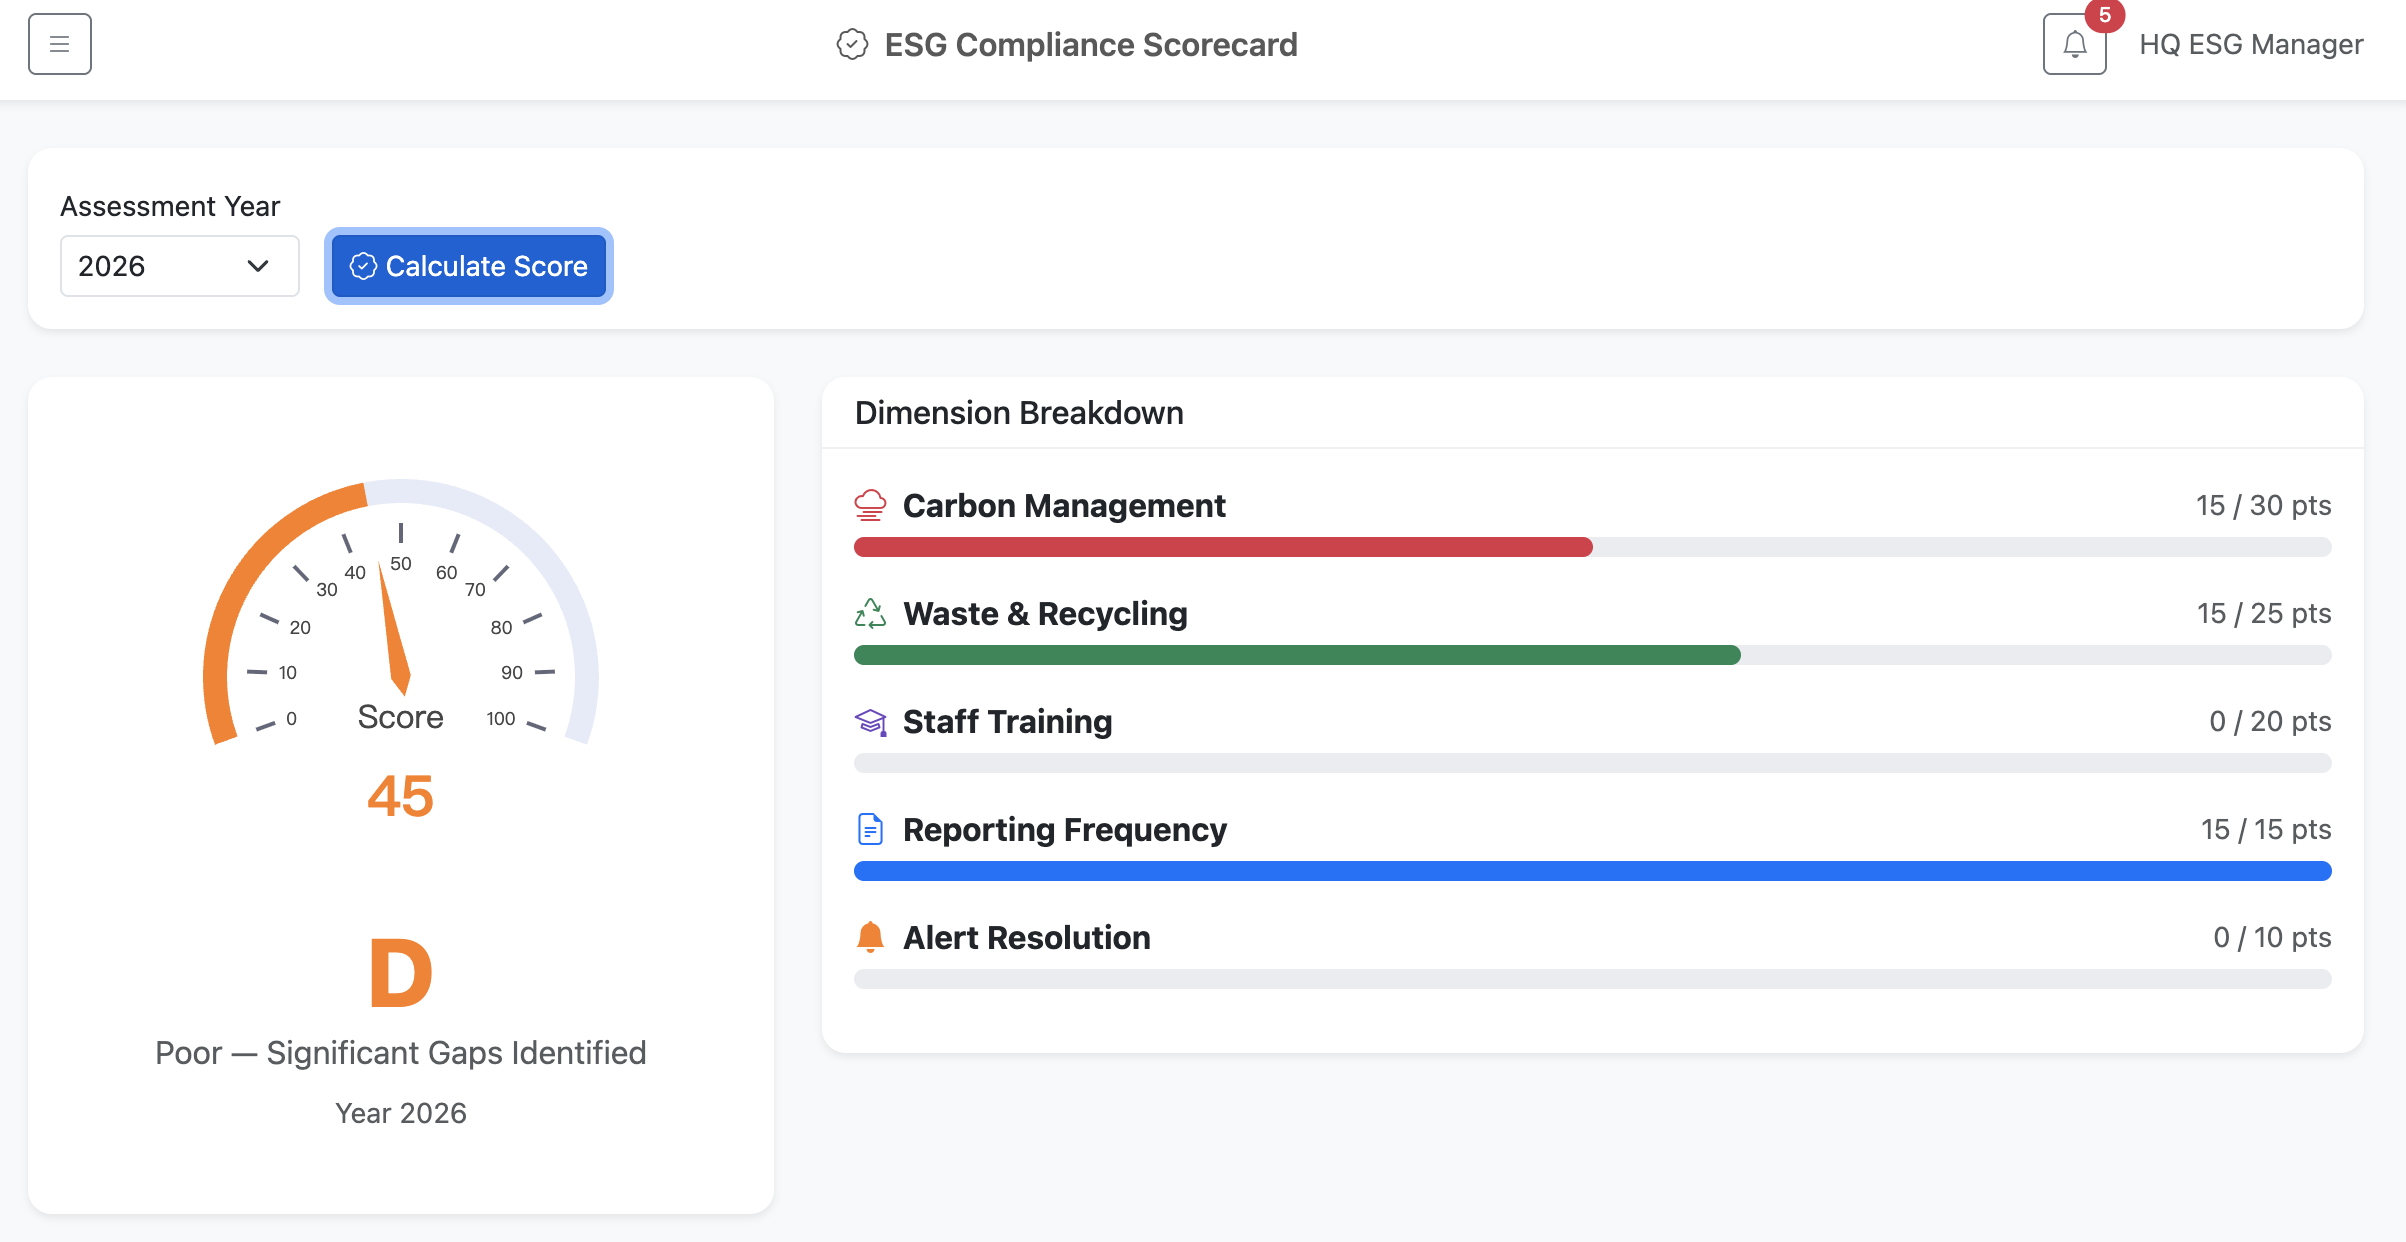
\includegraphics[width=0.65\textwidth]{compliance_score.png}
  \caption{Compliance Score page showing ESG scorecard and dimension breakdown}
  \label{fig:compliance_score}
\end{figure}

\subsection{Anomaly Detection}
The anomaly detection page helps users identify suspicious or abnormal carbon and waste values. This may include unusual spikes, implausible quantities, or records that fall far outside the normal range for a given store or period. When anomalies are detected, region managers should first verify the flagged record by cross-referencing the original data entry in the Carbon Tracking or Waste Management pages. If the record appears to be a genuine data error, they should contact the relevant store staff to correct or re-enter the data. Patterns of repeated anomalies for a specific store may warrant escalation to an HQ manager.

\begin{figure}[H]
  \centering
  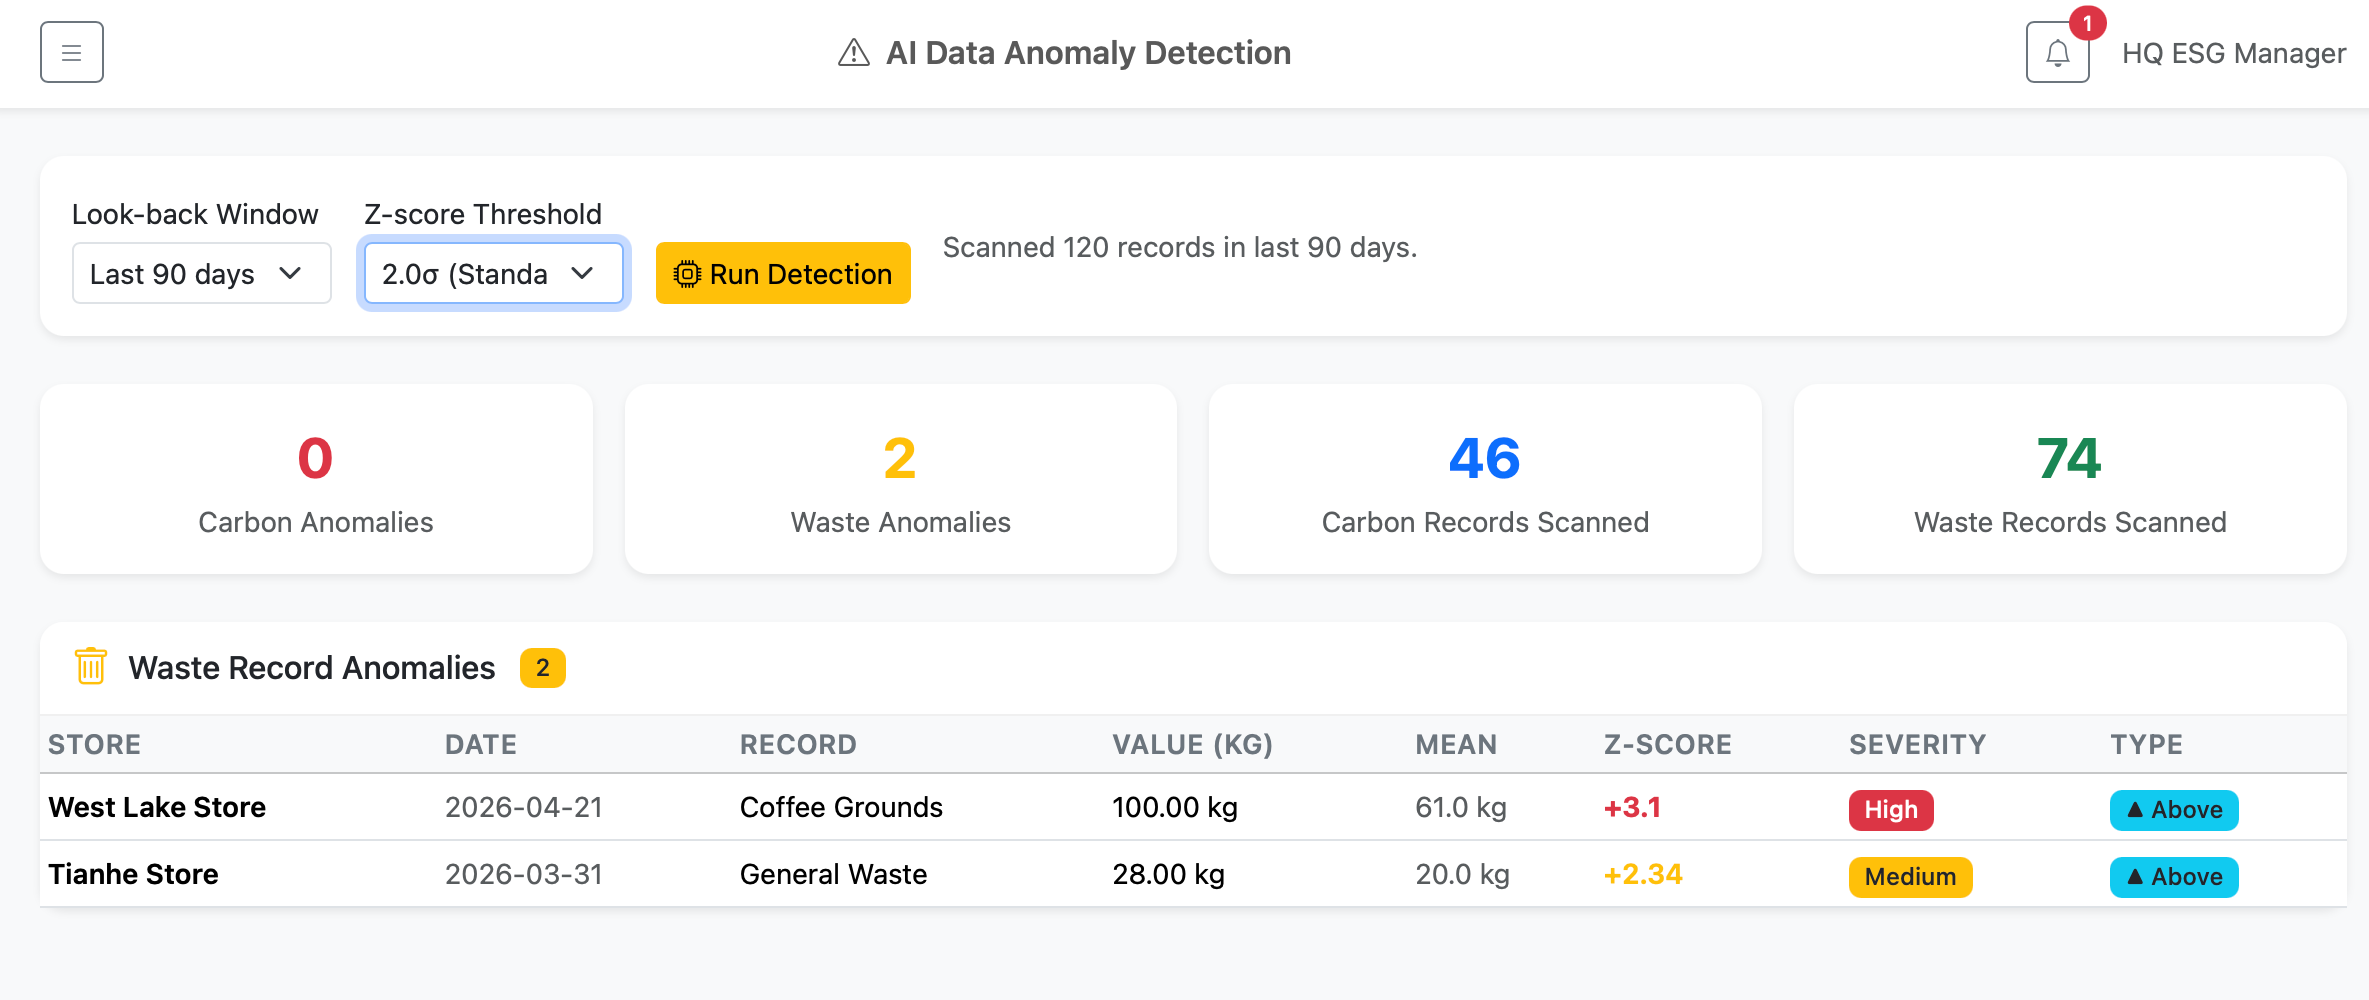
\includegraphics[width=0.80\textwidth]{anomaly_detection.png}
  \caption{Anomaly Detection page with flagged records}
  \label{fig:anomaly_detection}
\end{figure}

\section{HQ Manager and Admin Guide}

HQ managers and admins share access to the platform's most advanced management pages. After login, an HQ manager typically begins by reviewing the dashboard, then checks the Alerts page for any threshold breaches, reviews the Compliance Score page, and follows up with supplier ESG scores and internal policy status. Admins have the same access with broader authority -- they can manage users across the entire platform and are not restricted to a single company scope.

\subsection{Alert Threshold Configuration}
HQ managers can use the Alerts page -- the same page available to region managers for log review (Section~\ref{sec:region}) -- not only to review alert logs but also to define threshold rules. The threshold form includes metric type, condition, threshold value, scope, and optional notification email. This allows management to convert sustainability expectations into automated monitoring conditions.
\begin{figure}[H]
  \centering
  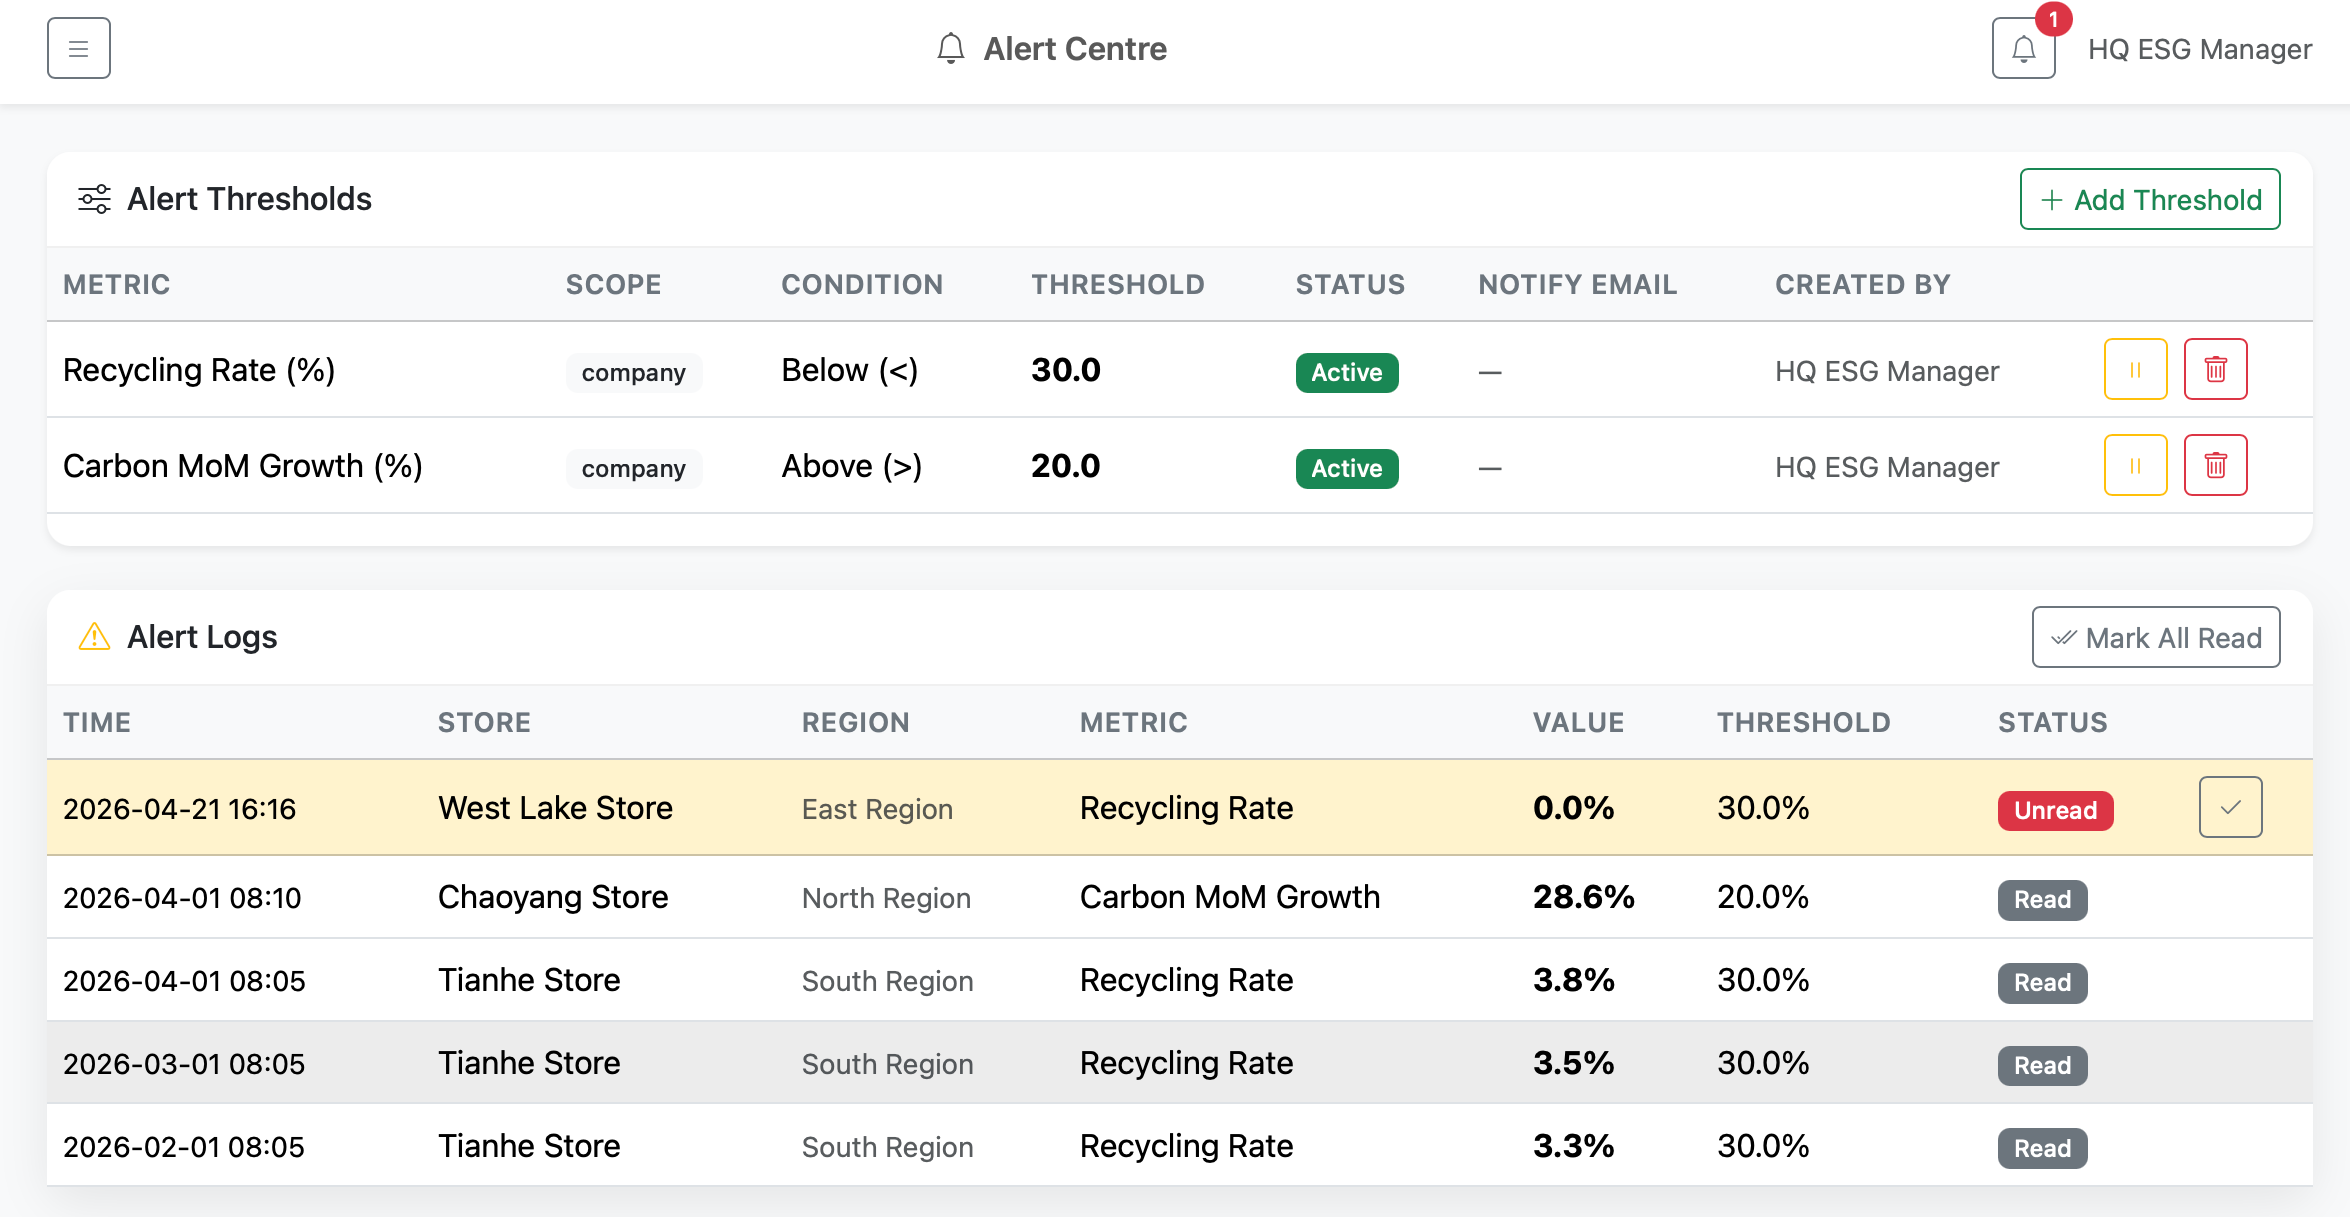
\includegraphics[height=5.5cm]{alert_page.png}
  \hfill
  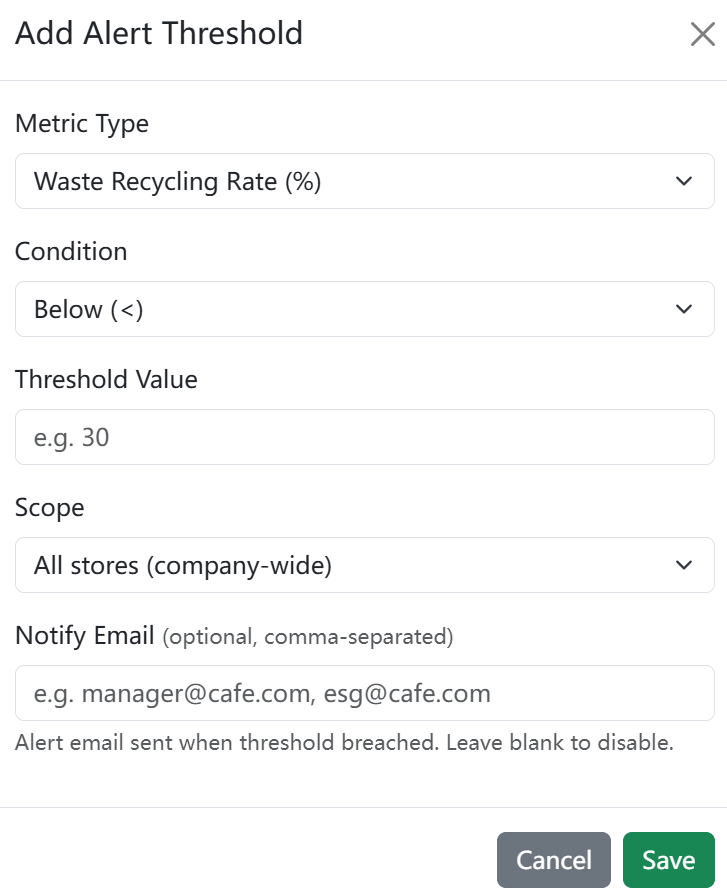
\includegraphics[height=5.5cm]{the Add Threshold modal.png}
  \caption{Alert Centre with active thresholds and logs (left) and threshold configuration form (right)}
  \label{fig:alerts-threshold}
\end{figure}


\subsection{Supplier ESG Assessment}
Within ESG Management, HQ managers can create and edit supplier records, as well as complete the ESG scorecard. Specifically, managers only need to select a score (from options of 0, 50, or 100) for each of the several sub-indicators, and the system will automatically calculate the dimension-level scores and the overall grade.
\begin{figure}[H]
  \centering
  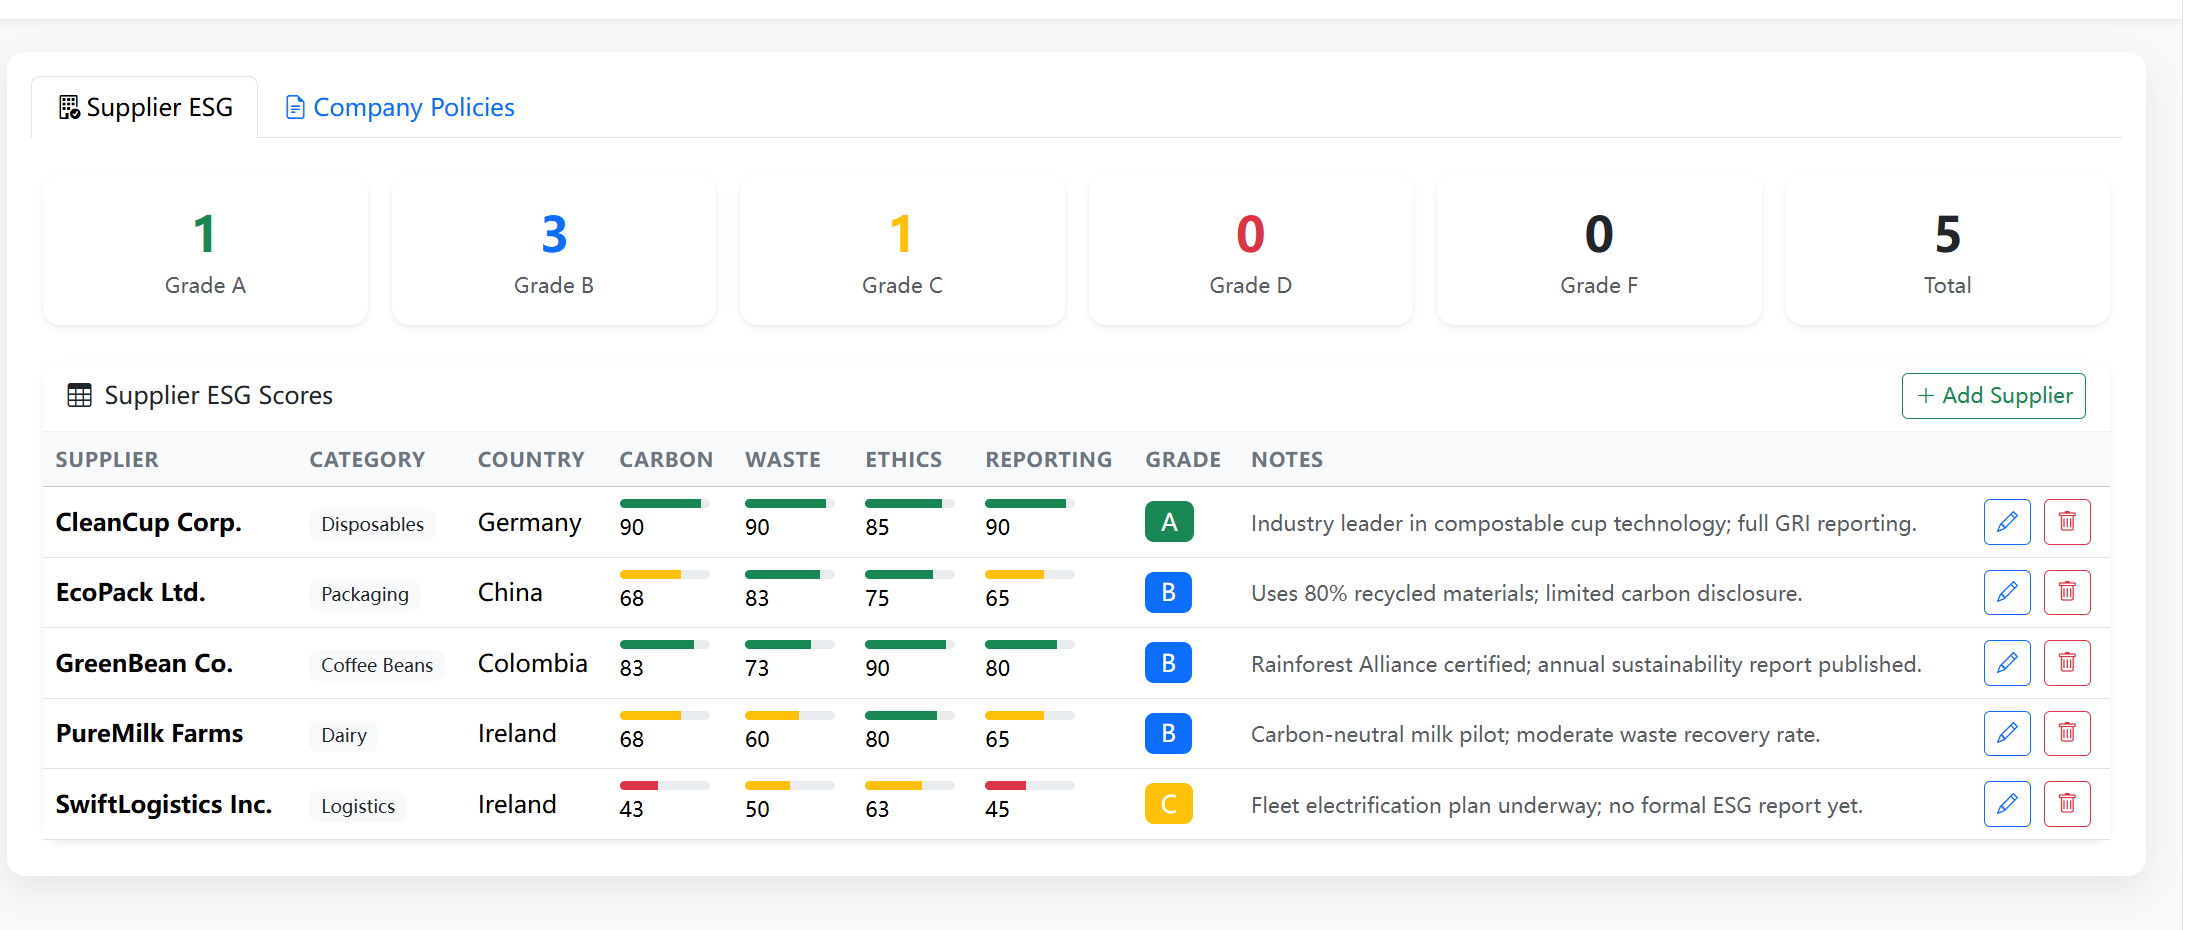
\includegraphics[height=4.5cm]{supplier ESG table with grades visible.png}
  \hfill
  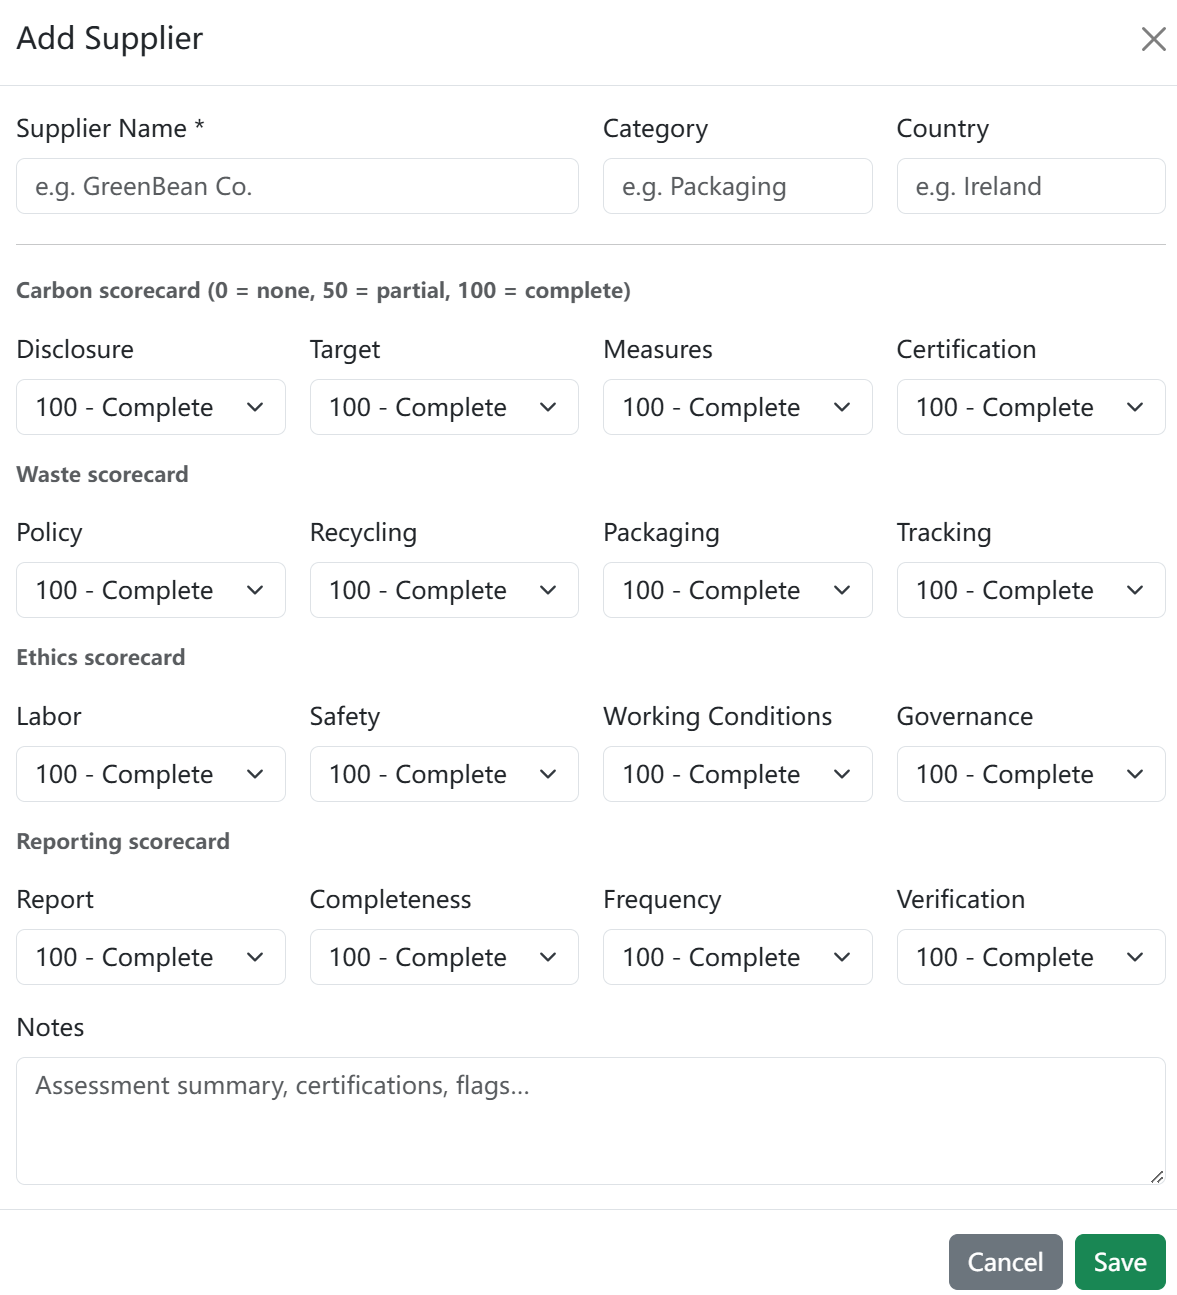
\includegraphics[height=4.5cm]{add and edit supplier modal showing scorecard.png}
  \caption{Supplier ESG assessment table (left) and scorecard entry form (right)}
  \label{fig:supplier-esg}
\end{figure}


\subsection{Company Policy Management}
The Policy tab is a lightweight internal document management page for ESG-related policies. Managers can create, edit, and delete policies, setting the title, category, status, effective date, version, and content. Each policy can be opened in a detail view, and an Edit button switches to the editing form.

\begin{figure}[H]
  \centering
  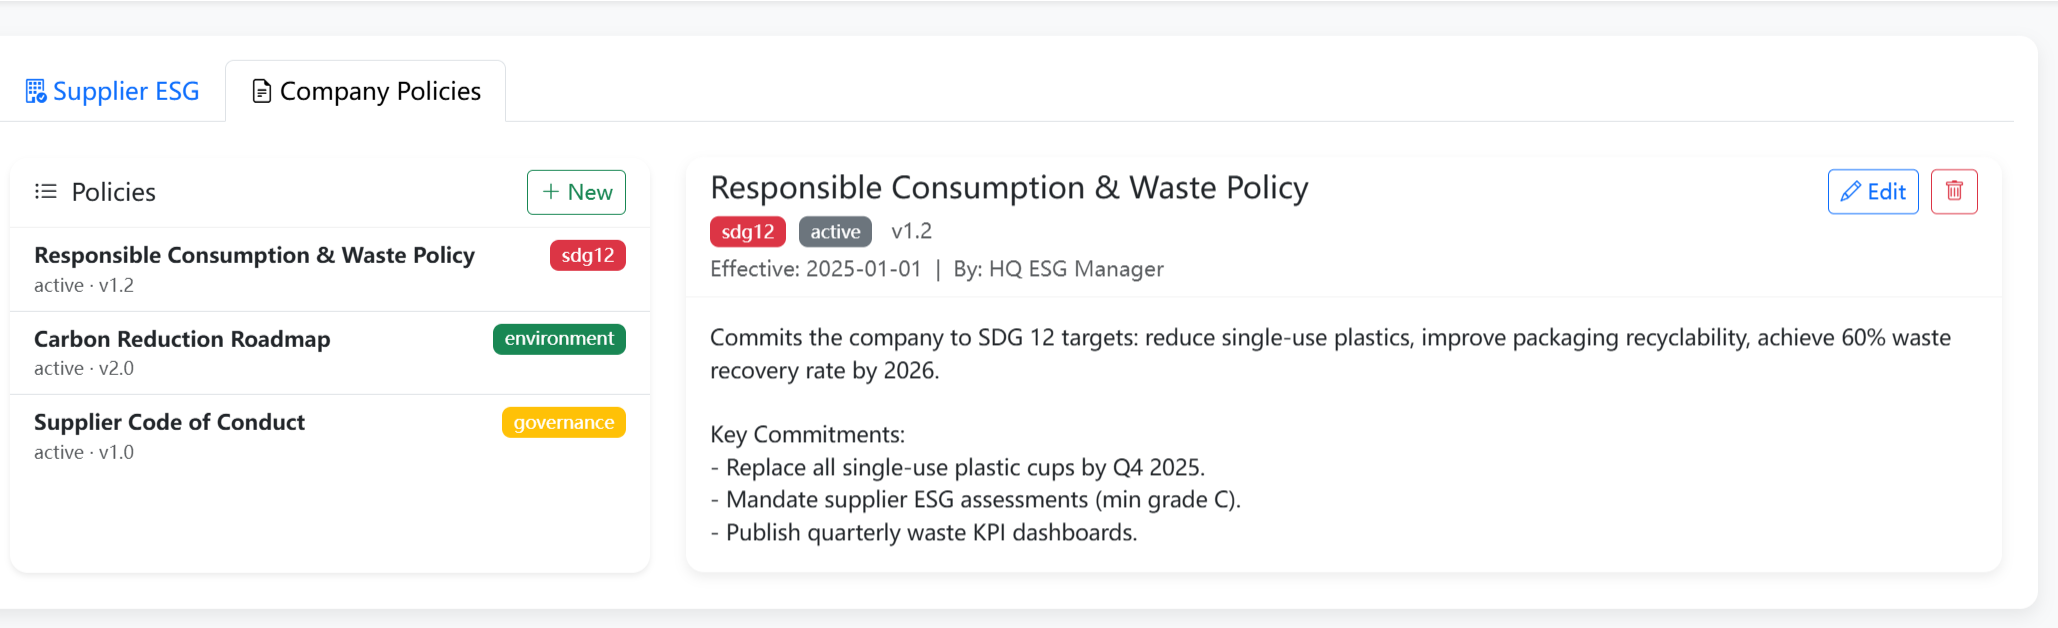
\includegraphics[width=0.78\textwidth]{the policy list.png}
  \caption{ESG policy management list}
  \label{fig:policy-list}
\end{figure}
  

\subsection{User Management}
The User Management page is accessible to HQ managers and admins. It provides summary cards for role distribution, a full user table with inline controls, and supports creating, editing, resetting passwords, and deleting accounts. Role and scope assignment -- including region and store fields -- can be configured when adding or editing a user.

\begin{figure}[H]
  \centering
  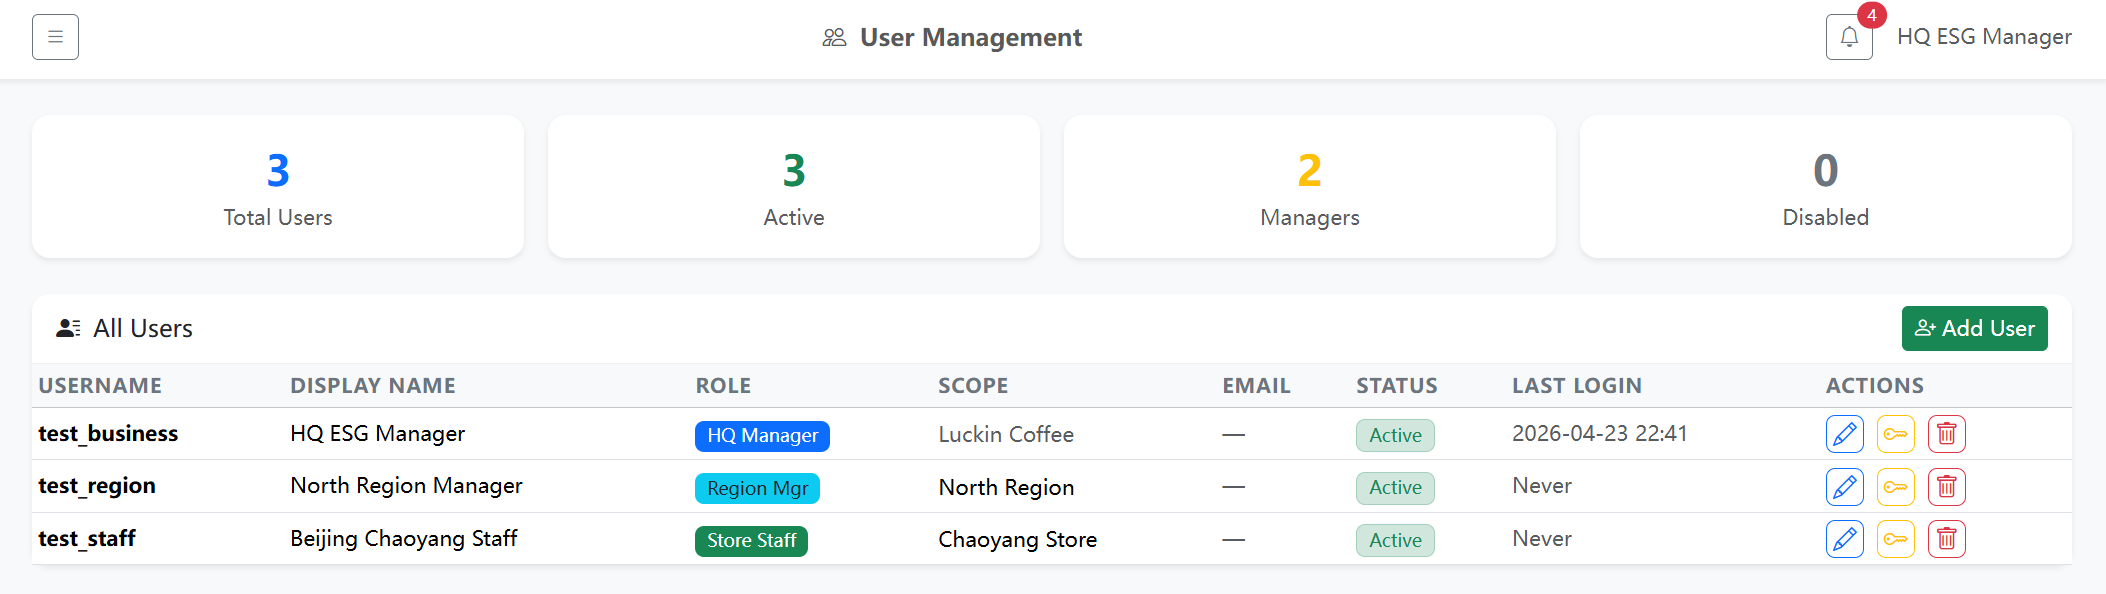
\includegraphics[width=0.88\textwidth]{main user table with summary cards.png}
  \caption{User management overview with role and scope summary cards}
  \label{fig:user-table}
\end{figure}


\subsection{Audit Log}
The Audit Log page enhances management visibility into critical system operations, with a focus on supporting review and accountability. It includes summary cards, filters, and an operation table that displays key details—including time, user, role, action, target, detail, and IP address—allowing managers to easily inspect and review system activity.
\begin{figure}[H]
  \centering
  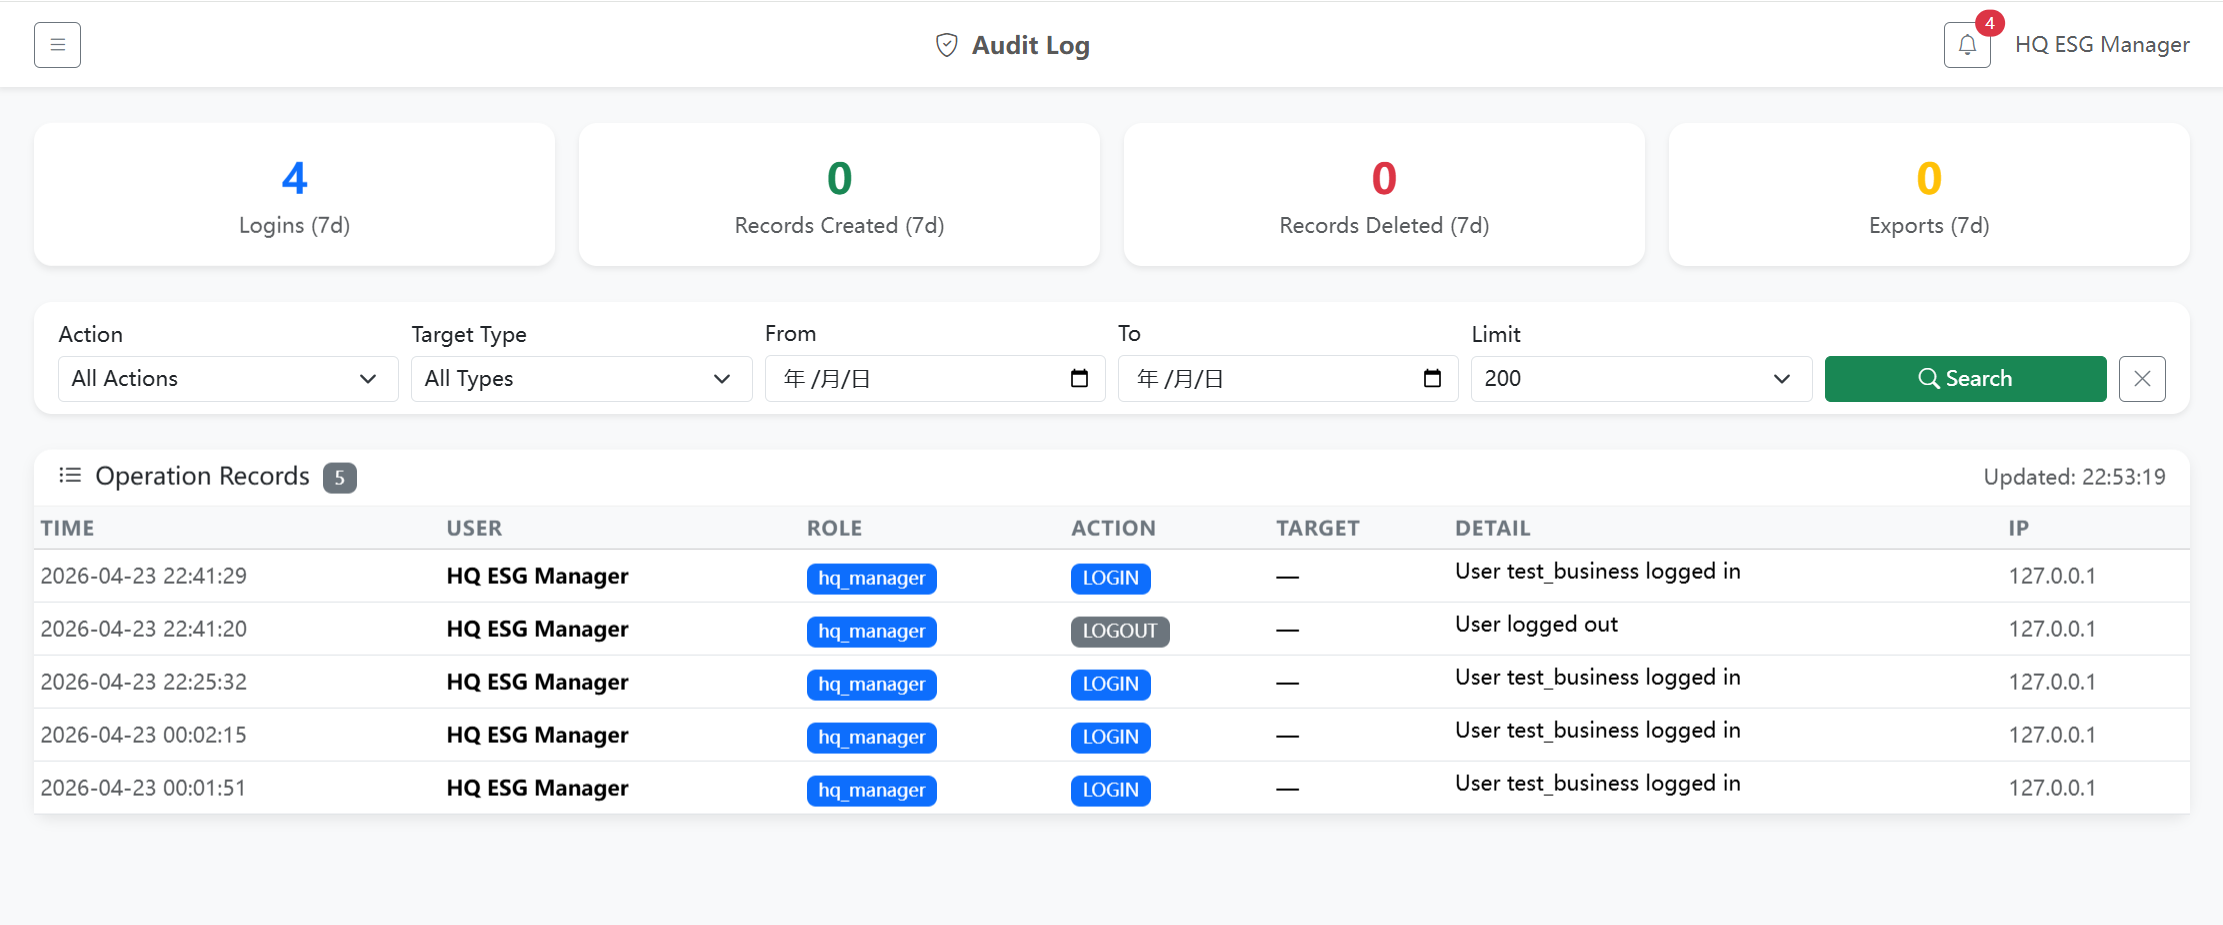
\includegraphics[width=0.65\textwidth]{the Audit Log page.png}
  \caption{Audit log with filters and activity table}
  \label{fig:audit-log-page}
\end{figure}

\section*{Conclusion}
This manual has covered the platform from login through to role-specific workflows, organised across four user types: Store Staff, Region Manager, HQ Manager, and Admin. Each role accesses a tailored set of pages, and the shared workflow sections in Section~4 provide the operational foundation that applies across all roles. Users conducting system testing should refer to the test accounts in Section 2.2 and follow the relevant role chapter as a step-by-step guide. The platform will continue to be updated, and this documentation will be revised accordingly throughout the project lifecycle.

\bibliographystyle{unsrtnat}
\bibliography{refs}

\end{document}
